\documentclass[12pt,letter]{article}
\usepackage[DIV=14,BCOR=2mm,headinclude=true,footinclude=false]{typearea}
\renewcommand{\baselinestretch}{1.15} 
\usepackage{latexsym}
\usepackage{amsmath}
\usepackage{MinionPro}
\usepackage{hyperref}
\usepackage{tikz}
\usepackage{verbatim}
\usepackage{natbib}
\usepackage{color, colortbl}
\usepackage{appendix}
\usepackage{amsmath,amsthm}


%\usepackage{wasysym}
%\usepackage{amssymb}

\usetikzlibrary{arrows,shapes}

\definecolor{Gray}{gray}{0.9}

\newtheorem{result}{Result}
\newtheorem{theorem}{Theorem}
\newtheorem{conjecture}{Conjecture}[section]
\newtheorem{corollary}{Corollary}[section]
\newtheorem{lemma}{Lemma}[section]
\newtheorem{proposition}{Proposition}[section]
\newtheorem{definition}{Definition}[section]
\newtheorem{assumption}{Assumption}[section]


\theoremstyle{definition}
\newtheorem{example}{Example}[section]

\theoremstyle{remark}
\newtheorem*{remark}{Remark}

\theoremstyle{claim}
\newtheorem{claim}{Claim}


\pgfdeclarelayer{background}
\pgfsetlayers{background,main}

\tikzstyle{vertex}=[circle,fill=black!25,minimum size=12pt,inner sep=0pt]
\tikzstyle{selected vertex} = [vertex, fill=red!24]
\tikzstyle{edge} = [draw,thick,-]
\tikzstyle{weight} = [font=\small]
\tikzstyle{selected edge} = [draw,line width=5pt,-,red!50]
\tikzstyle{ignored edge} = [draw,line width=5pt,-,black!20]


%\linespread{1.5}

\begin{document}
%\fontsize{12}{20pt}\selectfont

\title {Coordination in Social Networks}
\author {by Chun-Ting Chen}

\maketitle

\begin{abstract}

This paper studies a collective action problem in a setting of discounted repeated coordination games, where players only know their neighbors' types that describe the neighbors' inclination to participate and can only monitor their neighbors' past actions. I define \textit{strong connectedness} to say that, for every two players who incline to participate, there is a path consisting of players with the same types to connect them. Given that the networks are fixed, finite, connected, commonly known, undirected and without cycles, I show that if the state of nature has strong connectedness and if the priors have full support on the strong connectedness states, there is a (weak) sequential equilibrium in which the ex-post efficient outcome repeats after a finite time $T$ in the path when discount factor is sufficiently high. Given that the states of nature are finite and discrete, this equilibrium is constructive and does not depend on public or private signals other than players' actions.




\end{abstract}


\section{Introduction} 

This paper studies a collective action behavior in a setting of discounted repeated coordination games, where information and monitoring structures are modeled as networks. Players face the uncertainty about the states of nature and can only observe their neighbors' actions. I ask what kinds of networks can induce people to solve the underlying uncertainty and to coordinate to the ex-post efficient outcome. Though the main motivation is to understand the dynamic of social movement, a general interest is in the interaction between collective action behaviors and social structures.

Consider people's discontents in a rigid regime. Powerful discontents against this regime may exist, but these discontents are hard to put together due to the lack of complete information about how powerful they are and due to the communication barrier to know that these discontents exist. In the era of East German, the voting system and mass media are controlled by the government and the eavesdropping impedes people to show their political discontent\footnote{e.g., \citep{Lohmann2011}}. Before 1911 in China, several underground forces against Ching Dynasty scattered in the south of China, but they have different opinions of when and how to make a revolution, and the ways to communicate are dangerous. Though some social networks such as the networks of friends or organizations serve as routes in communication\footnote{e.g, \citep{Karl-Dieter1993}}, the communication is not free but costly in the sense that it is risky. While Berlin Wall became a history, we may then ask how a decisive collective action can be conducted with such information barrier. As social scientists have recognized it, the process of social movement can be traced back to periods ago, and an event can trigger another event\footnote{e.g., \citep{McAdamDoung;TarrowSidney;Tilly2001} \citep{McAdam2003} \citep{Lohmann2011}}. In game theory, a well-known feature in the extensive form incomplete information game is that the information sets a player faces are evolved with players' actions. When rebels know their actions can be used to transmit relevant information about how powerful this discontent is, they may be willing to take actions although taking actions is risky. I view such risky actions as parts of a equilibrium strategy and the entire movement as a learning process. 

I model such dynamic collective action in the following way. Players repeatedly play a $k$-\textit{Threshold game} with a parameter $k$ in a network. There are two types of players located in the network, one we called them \textit{Rebel} and one we called them \textit{Inert}.  Players' types and their actions can be observed {perfectly and only} by their neighbors\footnote{As \citep{chwe2000}.} . A Rebel has two actions, which are \textbf{revolt} or \textbf{stay}, while an Inert has only one action, which is \textbf{inert}. A Rebel will get pay-off as $1$ if he chooses \textbf{revolt} and more than $k$ players choose \textbf{revolt}; he will get pay-off as $-1$ if he chooses \textbf{revolt} and less than $k$ players choose \textbf{revolt}; he will get pay-off as $0$ if he chooses \textbf{stay}. An Inert will get pay-off as $1$ if he chooses \textbf{inert}.

Since a Rebel may not know how many Rebels in this world, Rebels' pay-off structure captures the idea that \textbf{stay} is a safe arm and \textbf{revolt} is a risky arm. Given a common prior $\pi$ over players' types, players play this $k$-Threshold game infinitely repeatedly with a common discount factor $\delta$. Cheap talk is not allowed, no outside mechanism serves as an information exchange device, and the static pay-off is unobservable\footnote{The assumption that the pay-off is hidden can be relaxed later in Section ~\ref{sec:varies}.}.

Rebels communicate with each other by playing actions. For different $k$ and different network structures, I am looking for a sequential equilibrium which has the property of \textit{approaching ex-post efficient} (APEX henceforth) to investigate such information sharing behavior in the networks. An equilibrium is APEX if and only if \textit{the tails of actions in the equilibrium path repeats the static ex-post efficient outcome after a finite time $T$}.  This refinement is to check if players learned the relevant information in the path. If there are at least $k$ Rebels in this society, then \textit{all} Rebels should \textbf{revolt} after $T$ by knowing that more than $k$ Rebels exist; otherwise, \textit{all} Rebels should \textbf{stay} after $T$. Rebels' incentives to communicate are affected by Rebels' positions in networks since the information structures are modeled as networks.

In order to get a quick intuition about Rebel's learning process in the proposed framework, consider the $k$-Threshold game with $k=n$. I.e. a Rebel can get positive pay-off only if all the players are Rebels. Assume that the networks are fixed, finite, connected, commonly known, and undirected (FFCCU henceforth), an APEX sequential equilibrium can be constructed by a contagion-like argument. This argument is to treat \textbf{stay} as the message of ``there is an Inert out there''; and treat \textbf{revolt} as the message of ``there could be no Inert out there ''. If I (a Rebel) have an Inert neighbor, then I play \textbf{stay} forever. If I have no Inert neighbors, then I play \textbf{revolt} until I observe that some of my neighbor play \textbf{stay}, and then I shift to play \textbf{stay} forever. Since the networks are FFCCU,  within finite periods, a Rebel will learn that there is an Inert out there if some neighbors has played \textbf{stay} and learn that there is no an Inert out there otherwise.

The non-trivial cases appear when $k<n$. The equilibrium construction when $k=n$ is simple because the binary actions, $\{\textbf{stay},\textbf{revolt}\}$, exactly separate the states into two parts, no Inerts or some Inerts. It is similar to the full-rank condition in which actions can generate distinguishable distribution of signals to tell the true states of nature\footnote{e.g., \citep{Fudenberg2010} or \citep{Fudenberg2011}.}. However, when $k<n$, such binary actions have to carry more informations to communicate such relevant information. As I will show them later, several sequences of actions will be used to transmit Rebels' private informations and to control Rebels' beliefs in equilibrium. In the equilibrium path, two kinds of sequence will be used. The first kind, \textit{reporting messages}, is to report the information about the state of nature; the second one, \textit{coordination messages}, is to report the information about whether some other Rebels have known such relevant information. The coordination message means to serve as a short-cut to bypass the tracking of individuals' higher-order beliefs about ``some Rebels have known the relevant information'', ``some Rebels have known some Rebels have known the relevant information'', etc.

Since playing \textbf{revolt} is not free but costly and since there is a discounting, Rebels always seek the opportunity to manipulate their messages to save their costs in the time horizontal line\footnote{Indeed, allowing cheap talk or using limit-of-mean preference (e.g., \citep{Renault1998}) will solve this coordination problem.}. As the problem will be cleared later, the usage of combinations of those two kinds of messages will incur a free rider problem happened locally aligned with the network structure. The intuition behind this is to see the forthcoming coordination as a public good that every Rebels can freely share with. This public good can only be made by Rebels' truthful reporting, which incurs some costs\footnote{Consider a situation where two nearby Rebels use reporting messages to exchange information. Suppose the relevant information can be revealed \textit{only} by them, and suppose \textit{every} Rebel can use a certain kind of coordination messages to trigger coordination \textit{no matter what} his past reporting messages are. In such case, then both players will shirk by not reporting anything to save their costs since they can wait for other's reporting, but then no one can learn the true relevant information.}.

In order to keep track the belief updating in the equilibrium path, a grim-trigger-like off-path belief will be used to enforce the strategies to follow prescribed forms of sequences. The criteria in judging a deviation need to be elaborated once the grim-trigger-like strategies are adopted. Some Rebels may fall outside a coordination with this grim trigger and therefore the APEX outcome can not be sustained. Because the pay-off function in our $k$-threshold game is not strictly increasing with the total number of Rebels' revolts, more than $k$ Rebels join an existing coordination did not change his pay-off. A Rebel may not have incentive to send messages to inform others to join an existing coordination since communication is always costly. 

The main result will show that this coordination problem can be solved in the FFCCU networks \textit{without cycles}. Here, I define the path in $G$ is a sequence consisting of nearby distinct nodes, and then I define a undirected network $G$ without cycles by defining a network in which the path between different nodes is unique. After I define \textit{strong connectedness} as the property that there is always a path consisting of Rebels to connect any pairs of Rebels,  the main result shows:

\begin{result}\textbf{Main Result}
In any FFCCU network without cycles, if the state has strong connectedness and if $\pi$ has full support on the strong connectedness states, then for $n$-person repeated $k$-Threshold game with parameter $1\leq k \leq n$, there is a $\delta$ such that a (weak) sequential equilibrium which is APEX exists.  
\end{result}




This paper contributes to several fields of economics. 

First, the future coordination can be viewed as a public good among all Rebels. A strand of public good literatures, such as \citep{Lohmann1994}, is to view information as a public good while generating information is costly\footnote{For instance, \citep{Lohmann1993}\citep{Lohmann1994} consider that individuals generate information by their actions, where their actions are public signals. \citep{Bolton1999} consider team experiment in infinite time horizon where the outcomes of experiments are public signals. \citep{Bramoulle2007} view information as a public good and consider public good provision in networks.}. This paper models costly information generation, while adding another aspect, network-monitoring, to investigate a collective action behavior.

Second, this paper is also related to the literature in social learning\footnote{Reviews can be seen in \citep{Bikhchandani1998} \citep{Cao2001}.}. Several papers have considered social learnings in networks \footnote{\citep{Goyal2012} gives the reviews. Recent papers, e.g., \citep{Acemoglu2011}\citep{Chatterjee2011}, also discuss this topic}. In these literatures, when players are myopic, the information flows could be very complicated because the information they sent can in turns affect their future behaviors\footnote{For example, in \citep{RePEc:eee:gamebe:v:45:y:2003:i:2:p:329-346},  even in a class of 3-person connected undirected network, the complete network and incomplete network will give different convergence results which highly depend on individuals' initial private signals and their allocations in a network. At least in \citep{Golub2010}, instead of using Bayesian learning, they use a naive learning protocol to tackle the learning problem in a network.}, and thus the learning results are hard to converge in the same way. This paper then consider the social learning in networks as a learning-in-game procedure, where individual can put more weights on the future learning results. My result give a hint that the shape of network (without cycle) did not matter too much if players are far-sighted.

Third, a growing literature consider the game played in networks where various games played in various networks by various definitions of networks\footnote{\citep{Jackson2008}\citep{Goyal2012} gives the reviews.}. Only few literatures among them discuss the repeated game. In complete information game. \citep{Laclau2012} proves a folk theorem where players play the game locally. \citep{Wolitzky2013} \citep{Wolitzky2014} consider network-like monitoring where a prisoner dilemma game played globally. This is the first paper to consider the incomplete information game repeatedly played in a network. 

The literatures in folk theorems in repeated game with incomplete information are also related. In those literatures, such as \citep{Fudenberg2010} \citep{Fudenberg2011} \citep{Wiseman2012}, they consider more general games than the games adopted here. However, as fas as my knowledge, a sufficient condition to show a folk theorem has not yet proposed to covered my setting\footnote{\citep{Fudenberg2010} \citep{Fudenberg2011} \citep{Wiseman2012} considering $n$-person game; \citep{Yamamoto2014} considering $2$-person game, they relies on the assumption on distribution of signals to inform players publicly or privately, which is the lack in my setting. An interesting result proposed by \citep{Amitai} can be also cited. \citep{Amitai} provide an example in $n$-person long cheap for incomplete information games. In that example, there is an incomplete information game such that if we enlarge the message space then the ex-post efficient outcome can be sustained, while limiting the message space will not sustain that outcome.}. I do not mean to prove a folk theorem here, my results however shows that the FFCCU networks without cycles are sufficient to sustain the ex-post efficiency when discount factor is sufficiently high. 

A final comment here is that the free rider problem may become more severe when a network has cycles. If a network has no cycles, a lemma in this paper will show that the potential free rider problems only happen locally between at most two nearby Rebels. However, when a network has cycles, there is an example to show that this problem can happen among more Rebels. I will discuss this problem later.

The paper is organized as the followings. Section ~\ref{sec:model} introduces the model. Section ~\ref{sec:equilibrium} discusses the equilibrium construction and shows the main result. Some variations will be discussed in its subsection ~\ref{sec:varies}. Section ~\ref{sec:con} makes the conclusion. All the missing proofs can be found in Appendix.

\section{Model}
\label{sec:model}
\subsection{Model}
Given a finite set $A$, denote $\#A$ as the cardinality of a set $A$, and denote $\Delta A$ as the set of probability distribution over $A$.

There are $n$ players. Denote $N=\{1,2,...,n\}$ as the set of players.  We say $G$ is a network if $G$ is a point-to-set function mapping from $N$ to a subset of $N$ containing $i\in N$. Moreover, we denote $G_i=G(i)$ as $i$'s neighbors and also denote $\bar{G}_i=G_i\backslash \{i\}$ as $i$'s neighborhood excluding $i$ self. We say $G$ is fixed if $G$ is not random, and say $G$ is undirected if for all $i,j$ if $j\in G_i$ then $i\in G_j$. Throughout this paper, I assume $G$ is finite, fixed, commonly known, and undirected. The set of states of nature is $\Theta=\{Rebel,Inert\}^n$ and let $\theta\in \Theta$ is a state of nature. For convenience, denote $[Rebels](\theta)=\{j:\theta_j=Rebel\}$ be the set of Rebels given $\theta\in \Theta$. Given $G$, let $p_{G_i}:\Theta \rightarrow 2^{\Theta}$ be $i$'s information partition function such that $p_{G_i}(\theta)=\Pi_{j\in G_i}\{\theta_j\}\times \{Rebel,Inert\}^{n-\#G_{i}}$. That is, whenever nature chooses a state, $i$ knows his own $\theta_i$ and his neighbor $j$'s $\theta_j$. 

There is a game, $k$-threshold game, infinitely repeated played with common discounted factor $\delta$ in a fixed $G$. Time is discrete, infinite horizontal. At the beginning of this game, a state is realized and there is a common prior $\pi\in \Delta \Theta$ over $\Theta$. After a state is realized, players simultaneously choose an action $a_{\theta_i}\in A_{\theta_i}$ in each period afterwards. If $\theta_i=Rebel$, then $A_{\theta_i}=\{\textbf{revolt}, \textbf{stay}\}$.  If $\theta_i=Inert$, then $A_{\theta_i}=\{\textbf{inert}\}$. Let $a_{\theta_i}\in A_{\theta_i}$ be $i$'s action if $i$'s type is $\theta_i$, and let $a_{-\theta_i}\in \Pi_{j\in N,j\neq i}A_{\theta_j}$ be the actions taken by players other than $i$. Player $i$'s static pay-off function, denoted as $u_{\theta_i}: \Pi_{j\in N}A_{\theta_j}\rightarrow \mathbb{R}$, in this $k$-threshold game is defined as followings. 
\begin{enumerate}
\item $u_{Rebel_i}(a_{Rebel_i},a_{-\theta_i})=1$ if $a_{Rebel_i}=\textbf{revolt}$ and $\#\{j:a_{\theta_j}=\textbf{revolt}\}\geq k$
\item $u_{Rebel_i}(a_{Rebel_i},a_{-\theta_i})=-1$ if $a_{Rebel_i}=\textbf{revolt}$ and $\#\{j:a_{\theta_j}=\textbf{revolt}\}< k$
\item $u_{Rebel_i}(a_{Rebel_i},a_{-\theta_i})=0$ if $a_{Rebel_i}=\textbf{stay}$
\item $u_{Inert_i}(a_{Inert_i},a_{-\theta_i})=1$ if $a_{Inert_i}=\textbf{inert}$
\end{enumerate}

The players can only observe the history of their neighbors' actions and the pay-off is hidden. Specifically, let $s$ be a period, and let $H^s_{G_i}=\prod^s_{t=0}\prod_{j\in G_i}A^s_{\theta_j}$ be the set of histories player $i$ can observe up to period $s$. Denote $H_{G_i}=\prod^{\infty}_{s=0}H^s_{G_i}$ be all the possible histories $i$ can observe. $i$'s pure behavior strategy is a sequence $\tau_{\theta_i}=(\tau^0_{\theta_i},...,\tau^s_{\theta_i},...)$, where $\tau^s_{\theta_i}: p_{G_i}(\theta)\times H^s_{G_i}\rightarrow A_{\theta_i}$ is a  measurable function with respect to $p_{G_i}(\theta)\times H^s_{G_i}$. For convenience, given $\theta$, also denote $\tau=\{\tau_{\theta_i}\}_i$,  $H^s=\prod^s_{m=0}\prod^n_{i=1}A_{\theta_i}$ and $H=\prod^{\infty}_{s=0}H^s$. The prior $\pi$, the network $G$, and strategies $\tau$ induce a joint distribution over $\Theta\times H$. 

Let 
$\beta^{\pi,\tau}_{G_i}(\theta|h^{s}_{G_i})$
be the conditional distribution over $\Theta$ conditional on $h^{s}_{G_i}\in H^s_{G_i}$ induced by $\tau$ for player $i$ at period $s$, and let
$E^{\delta}_G(u_{\theta_i}(\tau)|\beta^{\pi,\tau}_{G_i}(\theta|h^{s}_{G_i}))$
be the conditional expected pay-off conditional on $h^{s}_{G_i}$ for player $i$ with ${\theta_i}$.

We say a prior $\pi$ over a finite set has full support if  
\begin{definition}
$\pi$ has full support if and only if $\pi(\theta)>0$ for all $\theta\in \Theta$.
\end{definition}

The equilibrium concept here is the (week) sequential equilibrium. Given a network $G$, I am looking for a sequential equilibrium which is APEX. 

\begin{definition}\label{Def_expost_efficient}
A sequential equilibrium is APEX if and only if for all $\theta$ there is a finite time $T^{\theta}$ such that the tails of actions after $T^{\theta}$ in equilibrium path repeats the ex-post efficient outcome.
\end{definition}

In other words, in APEX, all the Rebels play \textbf{revolt} forever after some finite periods if there are more than $k$ Rebels; otherwise, Rebels play \textbf{stay} forever after some finite periods. The definition of APEX directly implies that Rebels must tell if there are more than $k$ Rebels or not in the equilibrium path as the following observation shows. This proof is in Appendix.

\begin{lemma}\label{lemma_learn}
Given $G$, $\pi$, $\delta$, $k$. If a sequential equilibrium $\tau^*$ is APEX, then given a $\theta$, there is a finite time $T_i$ for a Rebel $i$ such that $\sum_{\theta:\#[Rebels](\theta)\geq k}\beta^{\pi,\tau^*}_{G_i}(\theta|h^{s}_{G_i})$ either $=1$ or $=0$
whenever $s\geq T_i$.
\end{lemma}


The following example shows that an APEX can be founded if the $\delta$ is high enough. In this example, some Rebels play the roles as ``coordinators'' to reveal the relevant information to others.
\begin{example}\label{ex_leading_ex}
Suppose there are 3 players in a network.  This network is set as $G_1=\{1,2\}$, $G_2=\{1,2,3\}$,and $G_3=\{2,3\}$ as the following graph.

\begin{center}
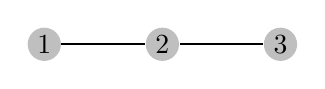
\begin{tikzpicture}[scale=1.5]
    % Draw a 7,11 network
    % First we draw the vertices
    \foreach \pos/\name in {{(1,0)/1}, {(2,0)/2}, {(3,0)/3}}
        \node[vertex] (\name) at \pos {$\name$};
    % Connect vertices with edges 
    \foreach \source/ \dest in {1/2, 2/3}
        \path[edge] (\source) -- (\dest) ;
        
\end{tikzpicture}
\end{center}

They are playing the $k$-threshold game with $k=3$ infinitely repeatedly. Note that after nature moves, player 2 can observe the true state of nature $\theta$, while player 1 or 3 are not. Player 2 plays the role as a coordinator. We can construct an equilibrium which is APEX as the followings. 

\begin{itemize}
\item After nature moves, Rebel 2 chooses $\textbf{revolt}$ if he observes $\theta=(Rebel,Rebel,Rebel)$, and plays \textbf{revolt} in this period. Otherwise, he chooses \textbf{stay} and keeps playing \textbf{stay} afterwards. 
\item After nature moves, Rebel 1 and Rebel 3 play \textbf{stay}.
\item If Rebel 2 chooses \textbf{revolt} in the last period, then Rebel 1 (or Rebel 3) plays \textbf{revolt} in this period; if Rebel 2 chooses \textbf{stay} in the last period, then Rebel 1 (or Rebel 3) keeps playing \textbf{stay} afterwards. 
\end{itemize}

Given the prior has full support, the above strategies constitute an equilibrium if $\delta\geq \frac{1}{2}$. In the equilibrium, Rebel 1 and Rebel 3 believe that $\{\theta:\#[Rebels](\theta)\geq 3\}$ with probability one if they observe that Rebel 2 has played \textbf{revolt} and believe $\{\theta:\#[Rebels](\theta)< 3\}$ with probability one if Rebel 2 has played \textbf{stay}.
\end{example}

In the following section, I begin to find an APEX equilibrium in a more general setting.

\section{Equilibrium}
\label{sec:equilibrium}
\subsection{The case: $k=n$}

In Example ~\ref{ex_leading_ex}, the construction of an APEX equilibrium relies on some important features. First, since $k=n$, Rebel 2 will never play \textbf{revolt} if one of his neighbor is Inert. Thus, when Rebel 2 plays \textbf{revolt}, it must be the case that all Rebel 2's neighbor are Rebels.  Second, Rebel 1 or Rebel 3 can force Rebel 2 to play \textbf{revolt} to reveal the true state in the first period since only Rebel 2 knows the true state and Rebel 2's actions can separate the states. Third, since $k=n$, one Rebel's shifting to play \textbf{stay} forever is enough to punish a deviation, and so that the group punishment is not necessary. For instance, if a Rebel did not play \textbf{revolt} in the first period at the state $\theta=(Rebel,Rebel,Rebel)$, his neighbor can punish him by playing \textbf{stay} forever. This punishment is credible by letting that player who deviated plays \textbf{stay} forever after he deviated. I then generalize the results for $k=n$ cases after one definition, \textit{connected}.

\begin{definition}
A path from $i$ to $j$, $i\neq j$ in an undirected network $G$ is a finite sequence $l_1,...,l_q$ such that $l_1=i, l_2\in \bar{G}_{l_1}, l_3\in \bar{G}_{l_2},...,l_q=j$ and $l_1,...,l_q$ are all distinct. An undirected network is connected if and only if for all $i,j$, $i\neq j$ there is a path from $i$ to $j$. 
\end{definition}



\begin{theorem}
\label{prop:not_crowded}
In any FFCCU network, if the prior has full support on $\Theta$, then for $n$-person repeated $k$-Threshold game with parameter $k=n$ played in such network,  there is a $\delta$ such that a sequential equilibrium which is APEX exists.
\end{theorem}
\begin{proof}
The proof is constructive and is a generalization of Example ~\ref{ex_leading_ex}. Let strategies $\tau^{*}$ as the followings. After nature moves, a Rebel play \textbf{revolt}  if there is no Inert neighbor; a Rebel play \textbf{stay} forever if there is a Inert neighbor. After first period, if a Rebel has not detected a deviation and if such Rebel observed his Rebel neighbor play \textbf{revolt} continuously in the last periods, then keep playing \textbf{revolt} in current period; otherwise, play \textbf{stay} forever. If a Rebel deviates, then he play \textbf{stay} forever.

According to $\tau^{*}$, at period $s$, if a Rebel has not detected a deviation and if such Rebel observed his Rebel neighbors have played \textbf{stay} once in the last periods, he forms belief $\sum_{\theta:\#[Rebels](\theta)\geq k}\beta^{\pi,\tau^*}_{G_i}(\theta|h^{s}_{G_i})=0$ after period $s$ and therefore plays \textbf{stay} after period $s$ is the best response. If a Rebel detects a deviation or himself deviate to play \textbf{stay}, play \textbf{stay} is the best response since at least one neighbor will play \textbf{stay}. 

Since the network is FFCCU, there is a finite time $t^{s}_{\theta}$ such that all Rebel play \textbf{revolt} forever if $\{\theta: \#[Rebels](\theta)\geq k\}$; and there is a finite time $t^f_{\theta}$ such that all Rebel play \textbf{stay} forever if $\{\theta: \#[Rebels](\theta)< k\}$ in the equilibrium path. If a Rebel deviates, he at most get 0 after $\max\{t^{s}_{\theta},t^f_{\theta}\}$, while he gets $\max\{1,0\}$ after $\max\{t^{s}_{\theta},t^f_{\theta}\}$. Due to the full support assumption, he will not deviate if $\sum_{\theta:\#[Rebels](\theta)\geq k}\beta^{\pi,\tau^*}_{G_i}(\theta|h^{s}_{G_i})>0$ at some period $s$, otherwise he has a loss in expected continuation pay-off by $\delta^{t^s_{\theta}}\frac{\sum_{\theta:\#[Rebels](\theta)\geq k}\beta^{\pi,\tau^*}_{G_i}(\theta|h^{s}_{G_i})}{1-\delta}$ after $t^s_{\theta}$. There is a $0<\delta_{\pi}<1$ such that he will not deviate.

To check if $\tau^{*}$ and $\{\beta^{\pi,\tau^*}_{G_i}(\theta|h^{s}_{G_i})\}_{i\in N}$ satisfy full consistency\footnote{Krep and Wilson (1982)}, take any $0<\eta<1$ such that Rebels play $\tau^{*}$ with probability $1-\eta$, and play others with probability $\eta$. Clearly, when $\eta \rightarrow 0$, the belief converges to $\{\beta^{\pi,\tau^*}_{G_i}(\theta|h^{s}_{G_i})\}_{i\in N}$.
\end{proof}



\subsection{The cases : $1<k<n$}

When $k<n$, the equilibrium constructed for the $k=n$ case will not work. First, a Rebel still has incentive to play \textbf{revolt} even if there is an Inert neighbor. Second, an Inert never transmit additional information about relevant information since they have only one action. We then require more assumptions on the states of natures and on the priors over the states of nature to get an APEX equilibrium. Example ~\ref{ex_strong_connectedness} shows why we need additional assumptions.

\begin{example}\label{ex_strong_connectedness}
Let $k=2$ and let the network as the following. Assume $\theta=(Rebel_1,Inert_2,Rebel_3)$.

\begin{center}
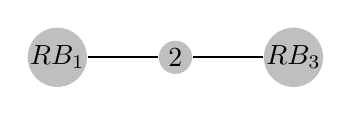
\begin{tikzpicture}[scale=1.5]
    % Draw a 7,11 network
    % First we draw the vertices
    \foreach \pos/\name in {{(1,0)/RB_1}, {(2,0)/2}, {(3,0)/RB_3}}
        \node[vertex] (\name) at \pos {$\name$};
    % Connect vertices with edges 
    \foreach \source/ \dest in {RB_1/2, 2/RB_3}
        \path[edge] (\source) -- (\dest) ;
        
\end{tikzpicture}
\end{center}

First, since $k=2$, Rebel 1 has incentive to play \textbf{revolt} when $\pi(\{\theta:\theta_3=Rebel\})$ is high enough given that player 3 will play revolt if himself is a Rebel. Second, Rebel 1 never learn $\theta_3$ since Inert 2 can not reveal information about $\theta_3$. We are now in the incomplete information game without communication. Clearly, an equilibrium which is APEX did not exist in this case.

\end{example}

In order to update Rebel's belief to get an equilibrium which is APEX (Lemma ~\ref{lemma_learn}), I narrow down the states of natures and the priors on them to avoid the cases as Example ~\ref{ex_strong_connectedness} shows. Define \textit{Strong connectedness} and \textit{Full support on strong connectedness} as the following.

\begin{definition}
\textbf{Strong connectedness}: Given $G$, a state $\theta$ has strong connectedness if and only if for every pair of Rebels, there is a path consisting of Rebels to connect them.
\end{definition}  

\begin{definition}
\textbf{Full support on strong connectedness}: Given $G$, $\pi$ has full support on strong connectedness if and only if $1>\pi(\theta)>0$ whenever $\theta$ has strong connectedness.
\end{definition}  


The goal of this paper is to show that a (weak) sequential APEX equilibrium always exists when $k<n$ in FFCCU networks without cycle given that $\delta$ is sufficiently high. I define cycles in FFCCU networks in the following definition and state my main theorem in Theorem ~\ref{thm_main_result}. 
\begin{definition}
A FFCCU network is without (with) cycles if and only if the path from $i$ to $j$, for $i\neq j$, is (is not) unique. 
\end{definition}

\begin{theorem}
\label{thm_main_result}
In any FFCCU network without cycles, if $\theta$ has strong connectedness and $\pi(\{\theta: \theta\text{ has strong connectedness}\})=1$ with full support on strong connectedness, then for $n$-person repeated $k$-Threshold game with parameter $1\leq k < n$ played in networks, there is a $\delta$ such that a (weak) sequential equilibrium which is APEX exists.
\end{theorem}

The equilibrium in Theorem ~\ref{thm_main_result} is constructive. I begin with an overview of equilibrium construction, and then illustrate such construction. The whole equilibrium strategies and the omitted proofs are all in Appendix.  

\subsubsection{Overview}

Given that the state has strong connectedness, Rebels have to find a way to communicate with each other. The construction of APEX is not trivial now because the ``dimension'' of information is generally larger than the cardinality of their own action space. Rebels then use several sequences of actions to transmit information, and thus we have to track the belief updating in the time horizontal line and to check if such sequences constitute an equilibrium. To see that Rebel need to communicate information with more dimensions, compare Example ~\ref{ex_cycle_number_5} and Example ~\ref{ex_cycle_number_6}.


\begin{example}\label{ex_cycle_number_5}
Let $k=5$ and let the network and the state $\theta$ as the following.

\begin{center} 
  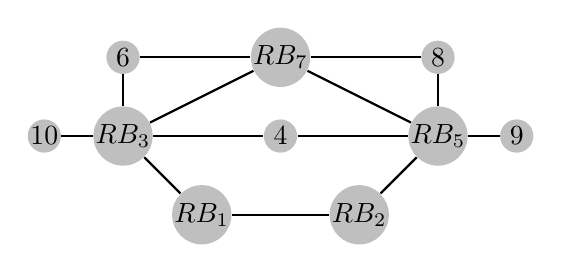
\begin{tikzpicture}[scale=1]
    % First we draw the vertices
    \foreach \pos/\name in {{(2,1)/RB_1}, {(4,1)/RB_2}, {(1,2)/RB_3}, {(5,2)/RB_5}, {(3,3)/RB_7}, {(3,2)/4}, {(1,3)/6}, {(5,3)/8}, {(6,2)/9}, {(0,2)/10}}
        \node[vertex] (\name) at \pos {$\name$};
        
%        \foreach \pos/\name in {{(3,2)/4_L}, {(1,3)/6_L}, {(5,3)/8_L}, {(6,2)/9_L}, {(0,2)/10_L}}
%   \node[selected vertex] (\name) at \pos {$\name$};
    
    % Connect vertices with edges 
    \foreach \source/ \dest in {RB_1/RB_2, RB_1/RB_3, RB_2/RB_5, RB_3/4, RB_3/6, RB_3/RB_7, 4/RB_5, RB_5/RB_7, RB_5/8, RB_5/9,6/RB_7, RB_7/8, RB_3/10}
        \path[edge] (\source) -- (\dest) ;
\end{tikzpicture}
\end{center} 

\end{example}


\begin{example}\label{ex_cycle_number_6}
Let $k=6$ and let the network and the state $\theta$ as the following.
\begin{center} 
  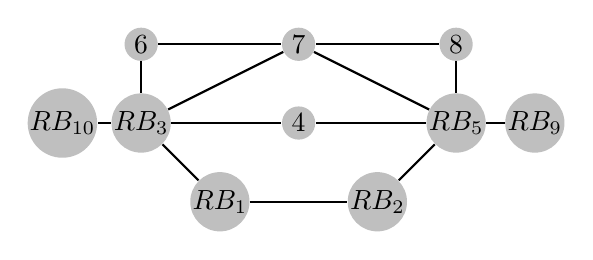
\begin{tikzpicture}[scale=1]
    % First we draw the vertices
    \foreach \pos/\name in {{(2,1)/RB_1}, {(4,1)/RB_2}, {(1,2)/RB_3}, {(5,2)/RB_5}, {(3,3)/7}, {(3,2)/4}, {(1,3)/6}, {(5,3)/8}, {(6,2)/RB_9}, {(0,2)/RB_{10}}}
        \node[vertex] (\name) at \pos {$\name$};
        
%        \foreach \pos/\name in {{(3,2)/4_L}, {(1,3)/6_L}, {(5,3)/8_L}, {(6,2)/9_L}, {(0,2)/10_L}}
%   \node[selected vertex] (\name) at \pos {$\name$};
    
    % Connect vertices with edges 
    \foreach \source/ \dest in {RB_1/RB_2, RB_1/RB_3, RB_2/RB_5, RB_3/4, RB_3/6, RB_3/7, 4/RB_5, RB_5/7, RB_5/8, RB_5/RB_9,6/7, 7/8, RB_3/RB_{10}}
        \path[edge] (\source) -- (\dest) ;
\end{tikzpicture}
\end{center} 


\end{example}

In Example ~\ref{ex_cycle_number_6}, there are 6 Rebels, while there are 5 Rebels in Example ~\ref{ex_cycle_number_5}. Suppose now we have a ``talking strategies''. Rebel 3 and Rebel 5 can talk about ``how many'' Rebels in their neighborhood to Rebel 1 and Rebel 2. Rebel 1 and Rebel 2 then talk with each other about ``how many'' Rebels they have known conditional on Rebel 3 and Rebel 5's taking. In some ways, Rebel 1 and Rebel 2 can initiate the coordination to play revolt conditional on `how many'' Rebels they have known. The question is that Rebel 1 and Rebel 2 still don't know how many Rebels out there after Rebel 3 and Rebel 5's talking since Rebel 3 and Rebel 5 will reveal the same number in both cases. Thus, ``talking about how many" nearby Rebels is not enough, Rebels have to ``talking about the locations'' of nearby Rebels to get APEX. 

Only having talking strategies to reveal both number and locations is, however, not enough to get APEX. Although Lemma ~\ref{lemma_learn} shows that there is a timing such that each Rebel have known the relevant information, but it did not characterize how Rebels have commonly known that. This higher-order information about ``Have there are some Rebels who have known relevant information?'' is an apparently giant object in the private monitoring setting. Here, Rebels use several ``coordination sequences'' to communicate this information by sending such sequences if they have known that some Rebels have known the relevant information.

I construct an APEX equilibrium with a weaker sequential consistent by assuming an off-path belief which has a grim-trigger property. More specifically, if a Rebel detect a deviation, he form the off-path belief as $\sum_{\theta \in \{\theta:\theta_j=Inert,j\notin G_i\}}\beta^{\pi,\tau}_{G_i}({\theta}|h^{s^{'}}_{G_i})=1$ for all $s^{'}\geq s$. I.e., a Rebel will think all players outside his neighborhood are Inerts and stop update his belief. Thus, if a Rebel has less than $k$ Rebel neighbors, he will play \textbf{stay} forever. 

The equilibrium is constructed by three steps as the following three subsections shows. In the first step, I define the \textit{information hierarchy in $G$} which gives a characterization to specify which Rebels have to report their information in equilibrium and gives the notations in constructing equilibrium. In second step, I show Rebels' strategies by showing the binary $\{\textbf{revolt},\textbf{stay}\}$-sequences used in equilibrium path and give the belief updating in the path. Finally, I discuss such grim-trigger-like off-path belief in the third step and give the idea of proof to show Theorem ~\ref{thm_main_result}. 

\subsubsection{Step 1. Information hierarchy in $G$}

The information hierarchy is defined on a network $G$ after nature chooses a state but before the game is played. I will use the term ``node $i$'' instead of ``player $i$'' in this step. 

The definition is by iteration. I define information hierarchy by defining $\{N^{-1}_i,N^{0}_i, N^{1}_i...\}$ and $\{I^{-1}_i,I^{0}_i, I^{1}_i...\}$ for each $i\in N$, and then define $\{\leq^0, \leq^1, \leq^2\}$ and $\{R^0,R^{1}, R^{2}...\}$ for each iteration in $(0,1,2,...)$. I also use the term ``blocks'' to represent the ``iterations''. 

Given $\theta$, the information hierarchy is defined as the followings.
\begin{itemize}

\item \textbf{0-block}
Denote
\begin{eqnarray*}
N^{-1}_i &\equiv &  i \\
I^{-1}_i & \equiv & i
\end{eqnarray*}

Then define $R^0$ as 
\begin{equation}
R^0\equiv\{i:\theta_i\in[Rebels](\theta)\}
\end{equation}

\item \textbf{1-block}
Denote
\begin{eqnarray*}
N^0_i &\equiv &  G_i \\
I^0_i & \equiv & G_i\cap R^0
\end{eqnarray*}

Define the set $\leq^0$ by defining
\begin{equation}i\in \leq^0 \Leftrightarrow \exists  j\in \bar{G}_i [I^0_i\subseteq N^0_j\cap R^0]\end{equation}  

Then define $R^1$ as 
\begin{equation}
R^{1} \equiv \{i\in R^0|i\notin \leq^0\}
\end{equation}

\item \textbf{$t+1$-block, $t\geq 1$}
Denote
\begin{eqnarray*}
N^t_i & \equiv & \bigcup_{k\in I^{t-1}_i}G_k \\
I^t_i & \equiv & \bigcup_{k\in G_i\cap R^t}I^{t-1}_k
\end{eqnarray*}


Define the set $\leq^t$ by defining
\begin{equation}i\in \leq^t \Leftrightarrow \exists j\in \bar{G}_i[I^t_i\subseteq N^t_j\cap R^0]\end{equation}

Then define $R^{t+1}$ as 
\begin{equation}
R^{t+1} \equiv  \{i\in R^t|i\notin \leq^t\}
\end{equation}


\end{itemize}

Thus, by examining the definition of $\leq^t$, the $R^t$ nodes are those nodes who have known some other Rebels but none of their neighbors have known these Rebels. Such nodes have the information at $t$-block, $I^{t-1}$, which contains the updating information about $\theta$. Since communication may incur expected costs, if a Rebel's private information can be fully reported by his neighbors and if there is no punishment, then he has no incentives to report it. Recall the Example ~\ref{ex_leading_ex}, there Rebel 2 is a $R^1$ node and Rebel 1 or 3 are not.

I characterize Rebels' incentives in this step, and let only $R^t$ nodes to report $I^{t-1}$ in next two steps. Moreover, if the networks are without cycles, Theorem ~\ref{lemma_empty} shows that it is sufficient to just let $R^t$ nodes to report information in the sense there is time $t$ and a $R^t$ node who will know the true state. 
\begin{theorem}
\label{lemma_empty}
If the network is FFCCU without cycle and if the state has strong connectedness, then 
\[R^0\neq \emptyset \Rightarrow \exists t\geq 0[\exists i\in R^t[I^t_i=R^0]]\]
\end{theorem}



\subsubsection{Step 2: Equilibrium strategies in the path}


Since Rebels need to communicate information with more dimensions, I assigned each player in a fixed network a distinguished prime number. Such indexation is starting from $3$. I index players $(1,2,...,n)$ as $(3,5,...,x_n)$ where $x_n$ is a prime number and the prime number assigned to $i$ will be $x_i$. Since the multiplication of distinguish prime numbers can be uniquely de-factorized as those numbers, I then use this property to let Rebels simultaneous report the number and the locations of their Rebel-neighbors by report the multiplication of those prime numbers.

I denote $\langle\rangle$ as a form of sequence. Denote $\bar{N}\subset N$ as an non-empty subset of $N$. The notations for the form of those sequences are shown in Table ~\ref{Table_msg_form}. 

\begin{table}[t]
\caption{Forms of sequences}
\label{Table_msg_form}
\begin{center}
\begin{tabular}{l c c}
$X_{\bar{N}}$ 								& $\equiv$ 			& $\prod_{j\in \bar{N}}x_j$  \\
\textbf{s}										& $\equiv$ 			& \textbf{stay}  \\
\textbf{r}										& $\equiv$ 			& \textbf{revolt}  \\
$\langle \textbf{stay} \rangle$ 		& $\equiv$ 			& $\langle \textbf{s},...,\textbf{s}\rangle$  \\
$\langle \textbf{revolt} \rangle$ 	& $\equiv$ 			& $\langle \textbf{r},...,\textbf{r}\rangle$  \\
$\langle  \bar{N} \rangle$ 				& $\equiv$ 			& $\langle \textbf{s},...,\textbf{s}\underbrace{\textbf{r},\textbf{s},...,\textbf{s}}_{X_{ \bar{N}}}\rangle$  \\

$\langle 1 \rangle$	 					& $\equiv$ 			& $\langle \textbf{s},...,\textbf{s}\underbrace{\textbf{r}}_{1}\rangle$  \\
$\langle \mathbf{1}_i \rangle$	 	& $\equiv$ 			& $\langle \textbf{s},...,\textbf{s}\underbrace{\textbf{r},\textbf{s},...,\textbf{s}}_{x_i}\rangle$  \\
\end{tabular}
\end{center}
\end{table}

Denote $|\langle\rangle|$ as the length of a form of finite sequence. The forms of sequences and the length of such forms will jointly determine the sequences I used in equilibrium. For example, if a sequence takes the form $\langle 1 \rangle$ and its length $|\langle 1 \rangle|=3$, then this sequence is $\langle \textbf{s},\textbf{s},\textbf{r}\rangle$. Note that the length of a form is calculate from the end of such sequence.

In the equilibrium path, two kinds of periods, \textit{reporting period} and \textit{coordination period}, occur in turns in the following way,
\[\underbrace{<\text{coordination period}>}_{0-block}\underbrace{<\text{reporting period}><\text{coordination period}>}_{1-block}...\]
I.e. after nature chooses a state, all the Rebels start with $0$-block, then enter to $1$-block,...,and so on. $0$-block has only one period, coordination period. The $t$-blocks, $t\geq 1$ has two periods, reporting period and coordination period, where reporting period occurs first and then coordination period follows. The length of each period in each block is finite but endogenous.

If a sequence of actions has been played in reporting period (or coordination period), I called it a \textit{reporting messages} (or \textit{coordination messages}). In reporting period in each $t$-block ($t\geq 1$), Rebels use the sequences defined in Table ~\ref{Table_msg_reporting} to report their $I^{t-1}_i$ contingent on the histories they observed. In coordination period in each $t$-block ($t\geq 0$), Rebels use the sequences defined in Table ~\ref{Table_msg_coordination} to check if there are some Rebels have known the relevant information, and then they either start to coordination to some actions after $t$-block or continue to enter next reporting period in $t+1$-block. I start to give the details of these messages.



\subsubsection*{Reporting messages in reporting period}

Denote $|\langle RP^t \rangle|$ be the total number of periods in $t$-block reporting period. I consider those pure strategies where the outcomes in equilibrium path take the following forms of sequences with length $|\langle RP^t \rangle|$ as Table ~\ref{Table_msg_reporting} shows. Any deviation from those forms in Table ~\ref{Table_msg_reporting} will be considered as a deviation. 

\begin{table}[ht]
\caption{Reporting messages}
\label{Table_msg_reporting}
\begin{center}
\begin{tabular}{c c }
Reporting Messages 		&   \\
\hline
$\langle  \textbf{stay} \rangle$ 	& 	 \\
$\langle  {I^{t-1}_i} \rangle$ 		&   \\
$\langle 1 \rangle$ 		             &    
\end{tabular}
\end{center}
\end{table}
In the equilibrium path, the beliefs a Rebel $j$ will form after observing his neighbor $i$'s reporting messages are shown in Table ~\ref{Table_blf_up_reporting}.

\begin{table}[ht]
\caption{Belief updating after reporting period}
\label{Table_blf_up_reporting}
\begin{center}
\begin{tabular}{l c l}
$i$ plays 		&  			& The events $j\in \bar{G}_i$ believe with probability one  \\
\hline
$\langle  \textbf{stay} \rangle$ 	& 			    & $i\notin R^t$  \\
$\langle  {I^{t-1}_i} \rangle$ 		&  			& $i\in R^t$ and $\theta_l=Rebel$ if $l\in I^{t-1}_i$      \\
$\langle 1 \rangle$ 		             &  			& $i\in R^t$ and $i$ has known $\#[Rebels](\theta)\geq k-1$ \\
\end{tabular}
\end{center}
\end{table}

Thus, Rebel can tell who are $R^t$ after reporting period. Recall that $R^t$ Rebels are those Rebels who have known some other Rebels any of their neighbors hasn't known, if a Rebel $j$ have observed that all of his neighbors are not in $R^t$, then he is sure that $\#[Rebels](\theta)< k$ if $\#I^{t-1}_j<k$. 

The important feature here is the usage of $\langle 1 \rangle$. It serve as a signal to indicate a pivotal player and to solve some potential free rider problems. I elaborate this issue here by providing some examples and give more details in the discussion for coordination period in next subsection. These problems happen when we allow a coordination message such that every Rebels can use regardless how their reporting messages. Consider the Example ~\ref{ex_free_rider_tree}.

\begin{example} \label{ex_free_rider_tree}\textbf{Free Rider Problem}

Let $k=5$ and assume that there are message $\langle M_4 \rangle,\langle M_5 \rangle$ for Rebel 4, 5. To simply the analysis, let the game play starting from $1$-block, i.e. by discarding the strategies in $0$-block and staring the game from the reporting period. Further, assume Rebels will play \textbf{revolt} forever after observing $\langle M_4 \rangle$ or $\langle M_5 \rangle$ being played once immediately after reporting period; otherwise they will play \textbf{stay} forever. Let $G$ be the followings.

\begin{center}
\begin{tikzpicture}[scale=1]
    % Draw a 7,11 network
    % First we draw the vertices
    \foreach \pos/\name in {{(1,2)/RB_1}, {(2,1)/RB_2}, {(2,3)/3}, {(3,2)/RB_4}, {(4,2)/RB_5}, {(5,1)/6}, {(5,3)/7}, {(6,2)/RB_8}}
        \node[vertex] (\name) at \pos {$\name$};
    
    
    % Connect vertices with edges 
    \foreach \source/ \dest in {RB_1/4, RB_2/RB_4,3/RB_4,RB_4/RB_5, RB_5/6, RB_5/7, RB_5/RB_8}
        \path[edge] (\source) -- (\dest) ;
        
\end{tikzpicture}
\end{center}

Note that Rebel 4 and Rebel 5 are $R^1$ members. Let $\langle \rangle_4$ and $\langle \rangle_5$ are the sequences of actions they may use to report the number of Rebel neighbors. If Rebel 5 report truthfully, then Rebel 4 will not report truthfully by arranging the occurrence of \textbf{revolt}s. Since Rebel 4 has a $\langle M_4 \rangle$ to initialize the coordination, such deviation is profitable. Same situation happens for Rebel 5, and then Rebel 4 and Rebel 5 will not report truthfully.

\end{example}

In the above example, two sources constitutes the free rider problem. One is that there is a coordination messages which can be used regardless the reporting messages. The other one is that Rebel 4 and Rebel 5 are \textit{pivotal} since they are sure that they will learn the true state given others' truthful reporting immediately after reporting period. To see the later source more clearly, consider the following Example ~\ref{ex_pivotal_1}.



\begin{example} \label{ex_pivotal_1}\textbf{Pivotal player: Case 1}
Let $k=6$ and suppose that there are message $\langle M_3 \rangle,\langle M_5 \rangle, \langle M_7 \rangle$ for Rebel 3,5,7 to initiate a coordination. Let the game play starting from $1$-block as Example ~\ref{ex_free_rider_tree}. Further, suppose Rebel will play \textbf{revolt} forever after observing $\langle M_3 \rangle$, $\langle M_5 \rangle$, or $\langle M_7 \rangle$ being played once in two periods immediately after this reporting period; otherwise they will play \textbf{stay} forever. Let $G$ be the followings.
\begin{center}
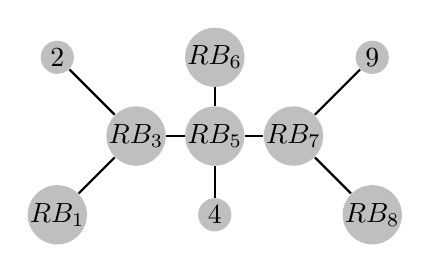
\begin{tikzpicture}[scale=1]
    % Draw a 7,11 network
    % First we draw the vertices
    \foreach \pos/\name in {{(1,1)/RB_1}, {(1,3)/2}, {(2,2)/RB_3}, {(3,1)/4}, {(3,2)/RB_5}, {(3,3)/RB_6}, {(4,2)/RB_7}, {(5,1)/RB_8}, {(5,3)/9}}
        \node[vertex] (\name) at \pos {$\name$};
    
    
    % Connect vertices with edges 
    \foreach \source/ \dest in {RB_1/RB_3, 2/RB_3,RB_3/RB_5,4/RB_5, RB_6/RB_5, RB_5/RB_7, RB_7/RB_8, RB_7/9}
        \path[edge] (\source) -- (\dest) ;
        
\end{tikzpicture}
\end{center}

Note that Rebel 3, 5, 7 are $R^1$ members. Differently from Example ~\ref{ex_free_rider_tree}, although Rebel 3, 7 have coordination messages, they still have incentives to report truthfully. This is because there is a possibility such that Rebel 5 will misunderstood the true state if they did not report truthfully to him, and they can not know the true state immediately after reporting period. Since the coordination to \textbf{revolt} has to be initiated immediately after this reporting period, they have incentives to report truthfully.

Rebel 5, however, has no incentive to report truthfully given others' truthful reporting since he is sure that he will know the true state immediately after reporting period.
\end{example}
   
Combine the discussions in Example ~\ref{ex_free_rider_tree} and Example ~\ref{ex_pivotal_1} , a way to deal with the free rider problem is to identify who is the pivotal player in the reporting period. If we can identify them, we can let them report nothing but sending the coordination messages. If the networks are FFCCU without cycles, Lemma ~\ref{lemma_at_most_two_nodes} shows that the free rider problem can be identified before the game enter to $t$-block and the pivotal player can be identified either. More precisely, first define $Tr_{ij}$ as a tree rooted in $i$ node while it leaves spanning from $j\in \bar{G}_i$.

\begin{definition}
$Tr_{ij}\equiv \{l\in N:\text{there is a unique path $\{l,...,j,i\}$ from $l$ to $i$ through $j$}\}$
\end{definition}
and define the set
\[C^t=\{i\in R^t:\nexists j\in R^{t-1}\cap \bar{G}_i[\exists l,l^{'}\in Tr_{ij}[l\in N^{t-1}_j\backslash I^{t-1}_i \text{ and } l^{'}\in \bar{G}_l]]\}\]
be those $R^t$ nodes such that there are no nodes connect with them by a path which has more than ``two walks''. For instance, the nodes Rebel 4 and Rebel 5 in Example ~\ref{ex_free_rider_tree} are $C^1$ nodes and Rebel 5 in Example ~\ref{ex_pivotal_1} is also a $C^1$ node. Then we can show the following lemmas. 

\begin{lemma}
\label{lemma_at_most_two_nodes}
If the network is FFCCU without cycle, and  if the state has strong connectedness, then for each $t$-block
\begin{enumerate}
\item $0\leq |C^t| \leq 2$.
\item Moreover, suppose there are two nodes in $C^t$, then they are each other's neighbor.
\end{enumerate}
\end{lemma}


\begin{lemma}
\label{lemma_no_node_outside}
If the network is FFCCU without cycle, and if the state has strong connectedness, then for each $t$-block
\[i\in C^t \Rightarrow \text{there is no node outside of }\bigcup_{k\in N^{t-1}_i}G_k\]
\end{lemma}

Lemma ~\ref{lemma_at_most_two_nodes} is crucial because a $C^t$ node can identify with each other by just checking the definition of $C^t$. If there are more than one $C^t$ nodes, we just pick a node who has smaller prime index to be a pivotal player\footnote{This property is not generally hold if a network has cycle.}. Lemma ~\ref{lemma_no_node_outside} characterize the intuition behind Example ~\ref{ex_free_rider_tree} and ~\ref{ex_pivotal_1}.

However, Lemma ~\ref{lemma_no_node_outside} does not show only the node in $C^t$ are pivotal. Some pivotal players thus can not be identified before the game enter $t$-block. Since that, we have to identify them during the game is played, and therefore we have to track their evolving information sets sequentially. This another source to let players become pivotal is that \textit{a Rebel has already known too much}, and therefore he is sure that he will learn {either $\#[Rebels](\theta)\geq k$ or $\#[Rebels](\theta)< k$} after current reporting period. Example ~\ref{ex_pivotal_2} give a concrete example.

\begin{example} \label{ex_pivotal_2}\textbf{Pivotal player: Case 2}
Let $k=6$. Again, assume that there are coordination message $\langle M\rangle$s for Rebels. Let the game play starting from $1$-block as Example ~\ref{ex_free_rider_tree}. Again, assume Rebel will play \textbf{revolt} forever after observing $\langle M \rangle$ being played once in four periods\footnote{It requires four periods to let the coordination message transmit.} immediately after reporting period; otherwise they will play \textbf{stay} forever. Let $G$ be the followings.

\begin{center}
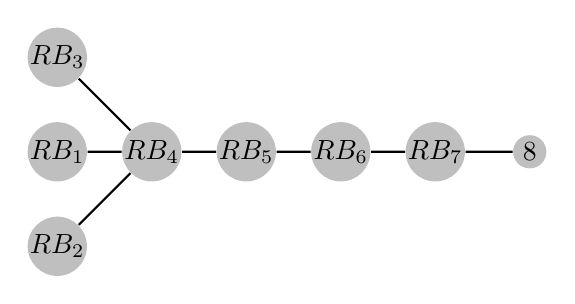
\begin{tikzpicture}[scale=1.2]
    % Draw a 7,11 network
    % First we draw the vertices
    \foreach \pos/\name in {{(2,2)/RB_1}, {(2,1)/RB_2}, {(2,3)/RB_3}, {(3,2)/RB_4}, {(4,2)/RB_5}, {(5,2)/RB_6}, {(6,2)/RB_7}, {(7,2)/8}}
        \node[vertex] (\name) at \pos {$\name$};
    
    
    % Connect vertices with edges 
    \foreach \source/ \dest in {RB_1/RB_4, RB_2/RB_4,RB_3/RB_4,RB_4/RB_5, RB_5/RB_6, RB_6/RB_7, RB_7/8}
        \path[edge] (\source) -- (\dest) ;
        
\end{tikzpicture}
\end{center}

In this case, no Rebels are in $C^1$, but Rebel 4 will deviate from reporting $\langle I^0_4 \rangle$. Note that Rebel 4 has already known there are 5 Rebels in this world, therefore knowing one more Rebels is enough to initiate the coordination to \textbf{revolt}. Moreover, if there is no more Rebels, the only coordination is the coordination to \textbf{stay}. If node 6 is a Rebel, Rebel 5 will report that, and therefore he will know $\#[Rebels](\theta)\geq 6$; Otherwise, due to the state has strong connectedness, he will also know $\#[Rebels](\theta)< 6$ for sure immediately after reporting period. Since he can use the message $\langle M \rangle$ to initiate the coordination, this deviation is profitable.
\end{example}

After the discussion in the above examples, the message $\langle 1 \rangle$ is introduced to specify the pivotal players. The pivotal players are those Rebels who have already known there are $k-1$ Rebels in the equilibrium path, or who are in $C^t$. The pivotal players will play $\langle 1 \rangle$ in the equilibrium path, and therefore the beliefs after observing $\langle 1 \rangle$ is that \textit{a Rebel has known $\#[Rebels](\theta)\geq k-1$} in the the path as Table ~\ref{Table_blf_up_reporting} shows.




\subsubsection*{Coordination messages in coordination period}

The ignorance of reporting messages after observed a coordination message $\langle M \rangle$ may incur untruthfully reporting as the above Example ~\ref{ex_free_rider_tree}, ~\ref{ex_pivotal_1}, and ~\ref{ex_pivotal_2} show, and the introducing of messages $\langle 1 \rangle$ is meant to tackle with this issue. However, one may have observed that the combination of these two messages, $\langle 1 \rangle\langle M \rangle$, themselves is another ``coordination message''. I.e., $\langle\langle \textbf{s}, \textbf{r} \rangle\langle M \rangle\rangle$ is another coordination message by truncating previous actions of $\langle 1 \rangle$ and concatenate the remaining to $\langle M \rangle$. If the contingent behavior after observing this new coordination message is the same as seeing the original one, $\langle M \rangle$, the untruthfully reporting problem has not been solved. In this section, I still let $\langle 1 \rangle$ as a reporting messages and call those $\langle M \rangle$ coordination messages, but I let the belief updating be contingent not only on the coordination messages but also on reporting messages.


There are three divisions in coordination period and there are several sub-blocks in each division. In $t=0$ block, the form is
\[\langle\underbrace{\langle \cdot \rangle }_{\text{$1$ sub-block}}\rangle \langle\underbrace{\langle \cdot \rangle }_{\text{$1$ sub-blocks}} \rangle \langle\underbrace{\langle \cdot \rangle \cdot \cdot \cdot \langle \cdot \rangle}_{\text{$n$ sub-blocks}}\rangle\] 
; in $t>0$ blocks, the form is
\[\langle\underbrace{\langle \cdot \rangle \cdot \cdot \cdot \langle \cdot \rangle}_{\text{$n$ sub-blocks}}\rangle \langle\underbrace{\langle \cdot \rangle \cdot \cdot \cdot \langle \cdot \rangle}_{\text{$t+1$ sub-blocks}} \rangle \langle\underbrace{\langle \cdot \rangle \cdot \cdot \cdot \langle \cdot \rangle}_{\text{$n$ sub-blocks}}\rangle\] 
, where $n=\# N$. 


Denote $CD^t_{m,q}$ be the $m$ sub-block in $q$ division, and denote $|\langle CD^t_{m,q} \rangle|$ be the total number of periods in $CD^t_{m,q}$.  The outcome of pure strategies in equilibrium path takes the following forms of sequences with length $|\langle CD^t_{m,q} \rangle|$ as Table ~\ref{Table_msg_coordination} shows.
\begin{table}[ht]
\caption{Coordination messages}
\label{Table_msg_coordination}
\begin{center}

\begin{tabular}{cc }
Coordination messages		&   \\
\hline
$\langle \mathbf{1}_i \rangle$ 	& 	 \\
$\langle \textbf{stay} \rangle$	&   \\
\textbf{r}									& 	\\
\textbf{s}									& 	\\
\end{tabular}
\end{center}
\end{table}

In the following paragraphs, I will focus on the behaviors in the coordination period in $t>0$ block, while Appendix shows the equilibrium path in coordination period in $t=0$ block. 

The belief a Rebel $j$ form after observing $i$ after $CD^t_{1,1}$ in equilibrium path is as Table ~\ref{Table_blf_up_cdt11} shows. After $CD^t_{1,1}$, Rebel $j$ will be notified one more event: $\#[Rebels](\theta)< k$. Clearly, $j$ will play \textbf{stay} forever if this event has been notified. In order to transmit this information about this event, Rebels will play $\langle \mathbf{1}_i \rangle$ unless they observe someone play $\langle \textbf{stay} \rangle$ in the path in $CD^t_{m,1}$ where $m\geq 2$ as Table ~\ref{Table_stg_cdt21} and Table ~\ref{Table_stg_cdtm1} shows. After $CD^t_{n,1}$, the information of $\#[Rebels](\theta)< k$ will be transmitted across all players. 
\begin{table}[ht]
\caption{Belief updating after $CD^t_{1,1}$, $t>0$}
\label{Table_blf_up_cdt11}
\begin{center}
\begin{tabular}{c c c}
In $RP^t$ 	&  	In $CD^t_{1,1}$		&  \\
\hline
\hline
$i$ plays 		&  	$i$ plays		& The events $j\in \bar{G}_i$ believe with probability one  \\
\hline
$\langle  \textbf{stay} \rangle$ 	& 	$\langle \mathbf{1}_i \rangle$	    & $i\notin R^t$ \\
$\langle  {I^{t-1}_i} \rangle$ 		&  $\langle \textbf{stay} \rangle$		& $\#[Rebels](\theta)< k$     \\
$\langle  {I^{t-1}_i} \rangle$ 		&  $\langle \mathbf{1}_i \rangle$		& $i\in R^t$     \\
$\langle 1 \rangle$ 		             &  $\langle \textbf{stay} \rangle$		& $\#[Rebels](\theta)< k$  \\
$\langle 1 \rangle$ 		             &  $\langle \mathbf{1}_i \rangle$		&  $\#[Rebels](\theta)\geq k$ 
\end{tabular}
\end{center}
\end{table}



\begin{table}[ht]
\caption{In-path strategies in $RP^t$, $CD^t_{1,1}$, and $CD^t_{2,1}$, $t>0$}
\label{Table_stg_cdt21}
\begin{center}
\begin{tabular}{c c c}
In $RP^t$ 	 	&  	In $CD^t_{1,1}$		&  In $CD^t_{2,1}$	\\
\hline
\hline
$i$ plays 		  							&  	$i$ plays									& $j\in \bar{G}_{i}$ plays  \\
\hline
$\langle  \textbf{stay} \rangle$ 	& 	$\langle \mathbf{1}_i \rangle$	    & $\langle \mathbf{1}_i \rangle$ \\
$\langle  {I^{t-1}_i} \rangle$ 		&  $\langle \textbf{stay} \rangle$		& $\langle \textbf{stay} \rangle$     \\
$\langle  {I^{t-1}_i} \rangle$ 		&  $\langle \mathbf{1}_i \rangle$		& $\langle \mathbf{1}_i \rangle$     \\
$\langle 1 \rangle$ 		             &  $\langle \textbf{stay} \rangle$		& $\langle \textbf{stay} \rangle$  \\
$\langle 1 \rangle$ 		             &  $\langle \mathbf{1}_i \rangle$		&  $\langle \mathbf{1}_i \rangle$  
\end{tabular}
\end{center}
\end{table}

\begin{table}[ht]
\caption{In-path strategies after $CD^t_{m,1}$, where $m\geq 2$, $t>0$}
\label{Table_stg_cdtm1}
\begin{center}
\begin{tabular}{c c c}
In $CD^t_{m,1}$, $m\geq 2$ 	 	&  	In $CD^t_{m+1,1}$,$m\geq 2$		& 	\\
\hline
\hline
$i$ plays 		  							&  $j\in \bar{G}_{i}$ plays  								& \\
\hline
$\langle \mathbf{1}_i \rangle$ 	& 	$\langle \mathbf{1}_i \rangle$	    &  \\
$\langle \textbf{stay} \rangle$		&  $\langle \textbf{stay} \rangle$	&  \\

\end{tabular}
\end{center}
\end{table}



Game enter to $CD^t_{1,2}$. In $CD^t_{1,2}$, Rebels start to check if the coordination to \textbf{revolt} can be initiated. The coordination message to initiate the coordination is $\langle \textbf{stay} \rangle$ as Table ~\ref{Table_blf_up_cdt12} shows. The important features here is that $\langle \textbf{stay} \rangle$ is a coordination message \textit{only if} $\langle  {I^{t-1}_i} \rangle$ or $\langle 1 \rangle$ has been played in reporting period.  First, note that $\langle \textbf{stay} \rangle$ is also the message to coordinate to \textbf{stay} in $CD^t_{m,1}$, $m\geq 1$ and note that this is the only candidate to be a message to coordinate to \textbf{stay}. Rebels are not confused about the information which \textbf{stay} carries since the information is now contingent on the reporting messages. Second, $\langle \textbf{stay} \rangle$ incurs no expected cost in equilibrium path. It is important because otherwise a free rider problem will happen again if such message incurs expected costs. Third, since this message is contingent on the reporting messages, initiating the coordination to \textbf{revolt} is ``not free'' since it requires Rebels to report something in reporting period to initiate that. This trade-off between reporting something and reporting nothing will force Rebels to report something in reporting period in order to take chances to initiate the coordination to \textbf{revolt}.

After the initiating in $CD^t_{1,2}$, Rebels start to transmit the information of $\#[Rebels](\theta)\geq k$ in $CD^t_{m,2}$ $m\geq 2$ as Table ~\ref{Table_stg_cdt12} and Table ~\ref{Table_stg_cdtm2} shows. That is, they will play $\langle \textbf{stay} \rangle$ unless they observe someone play $\langle \mathbf{1}_i \rangle$. After $CD^t_{{t+1},1}$, the information of $\#[Rebels](\theta)\geq k$ will be transmitted across at least $k$ Rebels. 

\begin{table}[ht]
\caption{Belief updating after $CD^t_{1,2}$, $t>0$}
\label{Table_blf_up_cdt12}
\begin{center}
\begin{tabular}{l c c c}
In $RP^t$ 	 	&  	In $CD^t_{1,1}$		&  In $CD^t_{1,2}$	  &\\
\hline
\hline
$i$ plays 		                             &  	$i$ plays		&				$i$ plays			& The events $j$ believe with probability one  \\
\hline
$\langle  \textbf{stay} \rangle$ 	& 	$\langle \mathbf{1}_i \rangle$	&  $\langle \textbf{stay} \rangle$ &  $i\notin R^t$ \\
$\langle  {I^{t-1}_i} \rangle$ 		&  $\langle \textbf{stay} \rangle$	&	$\langle \textbf{stay} \rangle$ &  $\#[Rebels](\theta)< k$   \\
$\langle  {I^{t-1}_i} \rangle$ 		&  $\langle \mathbf{1}_i \rangle$	&	$\langle \textbf{stay} \rangle$ &  $\#[Rebels](\theta)\geq k$    \\
$\langle  {I^{t-1}_i} \rangle$ 		&  $\langle \mathbf{1}_i \rangle$	&	$\langle \mathbf{1}_i \rangle$ &  $i\in R^t$  \\
$\langle 1 \rangle$ 		             &  $\langle \textbf{stay} \rangle$	&	$\langle \textbf{stay} \rangle$ &  $\#[Rebels](\theta)< k$\\
$\langle 1 \rangle$ 		             &  $\langle \mathbf{1}_i \rangle$	&	$\langle \textbf{stay} \rangle$ & $\#[Rebels](\theta)\geq k$
\end{tabular}
\end{center}
\end{table}




\begin{table}[ht]
\caption{In-path strategies in $RP^t$, $CD^t_{1,1}$, $CD^t_{1,2}$, and $CD^t_{2,2}$, $t>0$}
\label{Table_stg_cdt12}
\begin{center}
\begin{tabular}{l c c c}
In $RP^t$ 	 	&  	In $CD^t_{1,1}$		&  In $CD^t_{1,2}$	  & In $CD^t_{2,2}$ \\
\hline
\hline
$i$ plays 		                             &  	$i$ plays		&				$i$ plays			& $j\in \bar{G}_i$ plays  \\
\hline
$\langle  \textbf{stay} \rangle$ 	& 	$\langle \mathbf{1}_i \rangle$	&  $\langle \textbf{stay} \rangle$ &  $\langle \textbf{stay} \rangle$ \\
$\langle  {I^{t-1}_i} \rangle$ 		&  $\langle \textbf{stay} \rangle$	&	$\langle \textbf{stay} \rangle$ &  $\langle \textbf{stay} \rangle$   \\
$\langle  {I^{t-1}_i} \rangle$ 		&  $\langle \mathbf{1}_i \rangle$	&	$\langle \textbf{stay} \rangle$ &  $\langle \mathbf{1}_i \rangle$    \\
$\langle  {I^{t-1}_i} \rangle$ 		&  $\langle \mathbf{1}_i \rangle$	&	$\langle \mathbf{1}_i \rangle$ &  $\langle \textbf{stay} \rangle$  \\
$\langle 1 \rangle$ 		             &  $\langle \textbf{stay} \rangle$	&	$\langle \textbf{stay} \rangle$ &  $\langle \textbf{stay} \rangle$\\
$\langle 1 \rangle$ 		             &  $\langle \mathbf{1}_i \rangle$	&	$\langle \textbf{stay} \rangle$ & $\langle \mathbf{1}_i \rangle$
\end{tabular}
\end{center}
\end{table}

\begin{table}[ht]
\caption{In-path strategies after $CD^t_{m,2}$, where $m\geq 2$, $t>0$}
\label{Table_stg_cdtm2}
\begin{center}
\begin{tabular}{c c c}
In $CD^t_{m,2}$, $m\geq 2$ 	 	&  	In $CD^t_{m+1,2}$,$m\geq 2$		& 	\\
\hline
\hline
$i$ plays 		  							&  $j\in \bar{G}_{i}$ plays  								& \\
\hline
$\langle \mathbf{1}_i \rangle$ 	& 	$\langle \mathbf{1}_i \rangle$	    &  \\
$\langle \textbf{stay} \rangle$		&  $\langle \textbf{stay} \rangle$	&  \\

\end{tabular}
\end{center}
\end{table}






Game finally enter to $CD^t_{1,3}$. In this period, those $k$ Rebels who have known the information of $\#[Rebels](\theta)\geq k$ will start to play \textbf{revolt} forever, and this is the first period in the path in which a Rebel may get positive expected pay-off by playing \textbf{revolt}. After $CD^t_{m,3}$, $m\geq 2$, other Rebels start to transmit this information to all of the Rebels to coordinate to \textbf{revolt} as Table ~\ref{Table_stg_cdm3} shows.

\begin{table}[ht]
\caption{In-path strategies in $CD^t_{1,3}$, $t>0$}
\label{Table_stg_cd13}
\begin{center}
\begin{tabular}{c c c}
In $CD^t_{m,2}$, $1\leq m\leq t+1$ 	 	&  	In $CD^t_{1,3}$		& 	\\
\hline
\hline
$i$ has played 		  							&  $j\in \bar{G}_{i}$ plays  								& \\
\hline
$\langle \mathbf{1}_i \rangle$ 	& 	\textbf{r}	    &  \\
Otherwise		&  \textbf{s}	&  \\

\end{tabular}
\caption{In-path strategies after $CD^t_{m,3}$, where $m\geq 2$, $t>0$}
\label{Table_stg_cdm3}
\end{center}
\end{table}

\begin{table}[ht]
\begin{center}
\begin{tabular}{c c c}
In $CD^t_{m,3}$, $m\geq 2$ 	 	&  	In $CD^t_{m+1,3}$, $m\geq 2$		& 	\\
\hline
\hline
$i$ plays 		  							&  $j\in \bar{G}_{i}$ plays  								& \\
\hline
\textbf{r} 	& 	\textbf{r}	    &  \\
\textbf{s}		&  \textbf{s}	&  \\

\end{tabular}
\end{center}
\end{table}



\subsubsection{Step 3: Off-path Belief}

Whenever Rebel $i$ detects a deviation, he forms the belief 
\begin{equation}
\label{eq_grim_trigger}
\sum_{\theta \in \{\theta:\theta_j=Inert,j\notin G_i\}}\beta^{\pi,\tau}_{G_i}({\theta}|h^{s^{'}}_{G_i})=1
\end{equation}
for all $s^{'}\geq s$. Thus, if $\# I^0_i<k$, he will play \textbf{stay} forever and this is credible after $t$-block, $t>0$. This off-path belief then serve as a grim trigger to impede Rebels' deviation. 

As a discussion in Introduction, if the criteria in judging a deviation is too strict, an APEX equilibrium may not be sustained by using grim trigger. Due to the private monitoring structure, a deviation may be only detected by some Rebels while at least $k$ Rebels cannot detect it. Since that, at least $k$ Rebels may play \textbf{revolt} forever while the other Rebels may play \textbf{stay} forever if such judging is too strict. This phenomenon gives another reason why the message $\langle 1 \rangle$ is introduced. Example ~\ref{ex_deviation} (, a modification of Example ~\ref{ex_pivotal_1}) gives a concrete example to illustrate a case if $\langle 1 \rangle$ is not introduced, while this grim-trigger-like off-path belief is adopted. 

\begin{example}\label{ex_deviation}
Let $k=5$ and suppose that there are message $\langle M_3 \rangle,\langle M_5 \rangle, \langle M_7 \rangle$ for Rebel 3,5,7 to initiate a coordination. Let the game play starting from $1$-block as Example ~\ref{ex_pivotal_1}. Suppose Rebel will play \textbf{revolt} forever after observing $\langle M_3 \rangle$, $\langle M_5 \rangle$, or $\langle M_7 \rangle$ \textit{if no deviation be detected}; otherwise they will play \textbf{stay} forever. Moreover, assume that Rebels can only use the pure strategies in which the outcome satisfies the form of $\langle I^0_i \rangle$ in reporting period; \textit{otherwise, it  will be consider as a deviation}. 

Let the $G$ and $\theta$ be the following, and let the players be indexed by distinct prime numbers.

\begin{center}

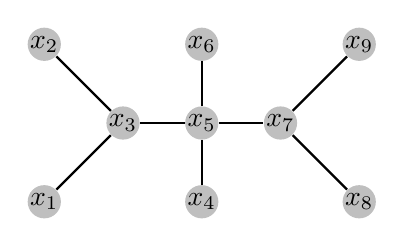
\begin{tikzpicture}[scale=1]
    % Draw a 7,11 network
    % First we draw the vertices
    \foreach \pos/\name in {{(1,1)/x_1}, {(1,3)/x_2}, {(2,2)/x_3}, {(3,1)/x_4}, {(3,2)/x_5}, {(3,3)/x_6}, {(4,2)/x_7}, {(5,1)/x_8}, {(5,3)/x_9}}
        \node[vertex] (\name) at \pos {$\name$};
    
    
    % Connect vertices with edges 
    \foreach \source/ \dest in {x_1/x_3, x_2/x_3,x_3/x_5,x_4/x_5, x_6/x_5, x_5/x_7, x_7/x_8, x_7/x_9}
        \path[edge] (\source) -- (\dest) ;
        
\end{tikzpicture}

\end{center}



\begin{center}
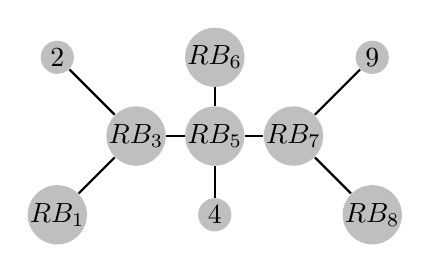
\begin{tikzpicture}[scale=1]
    % Draw a 7,11 network
    % First we draw the vertices
    \foreach \pos/\name in {{(1,1)/RB_1}, {(1,3)/2}, {(2,2)/RB_3}, {(3,1)/4}, {(3,2)/RB_5}, {(3,3)/RB_6}, {(4,2)/RB_7}, {(5,1)/RB_8}, {(5,3)/9}}
        \node[vertex] (\name) at \pos {$\name$};
    
    
    % Connect vertices with edges 
    \foreach \source/ \dest in {RB_1/RB_3, 2/RB_3,RB_3/RB_5,4/RB_5, RB_6/RB_5, RB_5/RB_7, RB_7/RB_8, RB_7/9}
        \path[edge] (\source) -- (\dest) ;
        
\end{tikzpicture}
\end{center}

Assume $X_{I^0_3}>X_{I^0_5}$ and $X_{I^0_7}>X_{I^0_5}$. Since that, Rebel 5 will get the information from Rebel 3,7 before he reports $I^0_5$. Since that, Rebel 5 has a profitable deviation by just reporting $\bar{I}^0_5=x_3\times x_5\times x_7<I^0_5$ to let Rebel 3, 7 think he is still in the path and to let the coordination to \textbf{revolt} be succeeded. Rebel 6 can detect such deviation since $\bar{I}^0_5$ did not include Rebel 6's own index $x_6$. However, if Rebel 6 form the off-path belief as Equation ~\ref{eq_grim_trigger}, he will then play \textbf{stay} forever although the coordination has been succeeded.

\end{example}

Due to the pay-off function is not strictly increasing with the number of \textbf{revolts}, some Rebels will be excluded from coordination with this grim-trigger-like strategies. As Example ~\ref{ex_deviation} shows, some strategies other than $I^t$ have to be considered as the strategies in the equilibrium path to avoid the situation where some Rebels are out of an existing coordination. The introducing of message $\langle 1 \rangle$ gives more equilibrium paths when grim trigger is adopted. 

\subsubsection{Sketch of the proof for Theorem ~\ref{thm_main_result}}

In previous subsections, I have listed the belief updating in equilibrium path by showing the the belief updating after observing various messages. Lemma ~\ref{lemma_in_the_path} show that the equilibrium path is APEX where the consistent in-path belief updating is listed in Table ~\ref{Table_blf_up_reporting}, ~\ref{Table_blf_up_cdt11}, and ~\ref{Table_blf_up_cdt12}. 
\begin{lemma}\label{lemma_in_the_path}
If the state has strong connectedness, then for all $n$-person repeated $k$-Threshold game with parameter $1\leq k\leq n$ played in any FFCCU network without cycles, the equilibrium is APEX.
\end{lemma}

For the histories outside of equilibrium path, they could be detectable or undetectable. The argument to prove Theorem ~\ref{thm_main_result} is as the following. First, I use off-path belief to prevent players from making detectable deviations, such as deviations from playing the specified forms of sequences listed in Table ~\ref{Table_msg_reporting} and ~\ref{Table_msg_coordination}. Then I argue that any undetectable deviation made by a Rebel before he knows the relevant information, $\#[Rebels](\theta)\geq k$ or $\#[Rebels](\theta)< k$, will create noises in his own learning process and then reduce his own expected continuation pay-off.  To see why making undetectable deviation will create noises to impede the learning process before he knows the relevant information, consider the case when a Rebel wants to mimic pivotal plays' behaviors by sending $\langle 1 \rangle$. According to Table ~\ref{Table_blf_up_cdt11} and Table ~\ref{Table_blf_up_cdt12}, the continuation playing by his neighbors after observing $\langle 1 \rangle$ is to play \textbf{stay} forever or to play \textbf{revolt} forever. Since all his neighbors repeats the same action, he can not learn additional information about $\theta$. When $\delta$ is high enough, since he can learn the relevant information by Lemma ~\ref{lemma_learn} if he stay in the path, he is better off by staying in the equilibrium path to achieve the maximum static pay-off as 1 when $\#[Rebels](\theta)\geq k$ and achieve the maximum static pay-off as 0 when $\#[Rebels](\theta)< k$. Claim ~\ref{claim_can_not_pretend_almost_success} shows this argument.

\subsection{Discussion}
\label{sec:varies}


\subsubsection{Variation: Pay-off as signals}
The assumption on the observability of pay-off can be relaxed without change the result in Theorem ~\ref{thm_main_result}. One may consider a situation such that the static pay-off depends not only on joint efforts but also depends on other random effects, says the weather.\footnote{e.g.,\citep{SHADMEHR2011}}. Specifically, consider there is a public signal $y\in \{y_1,y_2\}$ generated by Rebels' actions. Let Rebel $i$'s pay-off function be $u_{Rebel}(a_{Rebel_i},y)$, and let $u_{Rebel}(\textbf{stay},y_1)=u_{Rebel}(\textbf{stay},y_2)=u_0$. The distribution of $y_1$ and $y_2$ is 
\begin{eqnarray*}
p_{1s} &=& \mathrm {Pr}(y=y_1|\#\textbf{revolt}\geq k) \\
p_{1f} &=& \mathrm {Pr}(y=y_1|\#\textbf{revolt}< k) \\
p_{2s} &=& \mathrm {Pr}(y=y_2|\#\textbf{revolt}\geq k) \\
p_{2f} &=& \mathrm {Pr}(y=y_2|\#\textbf{revolt}< k) 
\end{eqnarray*}
with
\begin{equation}
p_{1s}u_{Rebel}(\textbf{revolt}, y_1)+p_{2s}u_{Rebel}(\textbf{revolt}, y_2)>u_0>p_{1f}u_{Rebel}(\textbf{revolt}, y_1)+p_{2f}u_{Rebel}(\textbf{revolt}, y_2)
\end{equation}
and
\begin{equation}
1>p_{1s}>0,1>p_{2s}>0,p_{1f}=1-p_{1s},p_{2f}=1-p_{2s}
\end{equation}

Equation (6) is a generalization for the previous setting. Equation (7) is a full support assumption on signal $y$. 

We can construct exactly the same equilibrium strategies by ignoring the noisy signal $y$ when Equation (7) holds. By directly checking the equilibrium path constructed in previous sections (see also Table ~\ref{Table_msg_reporting} and ~\ref{Table_msg_coordination}), \textit{at most one} Rebel playing \textbf{revolt} in a period before some Rebels play $\langle 1 \rangle$, and thus the signal $y$ is not relevant before some Rebels play $\langle 1 \rangle$. Moreover, playing $\langle 1 \rangle$ comes from a Rebel's observation in reporting period where Rebels' strategies are independent from $y$, and thus playing $\langle 1 \rangle$ is independent from $y$. We then just check if a Rebel want to deviate to play $\langle 1 \rangle$ to get additional information coming from $y$. According to equilibrium strategies in the path, however, playing $\langle 1 \rangle$ will incur either coordination to \textbf{stay} or coordination to \textbf{revolt} after current block as Table ~\ref{Table_blf_up_cdt11} and Table ~\ref{Table_blf_up_cdt12} shows. Since signal $y$ is noisy, and since Rebels' actions will repeat, he can not learn the relevant information. As the same argument in Claim ~\ref{claim_can_not_pretend_almost_success}, he is better off by staying in the equilibrium path.

If Equation (7) fails, and so that the signal $y$ is not noisy, says $p_{1s}=p_{2f}=1$, the equilibrium constructed in the previous section is no longer an equilibrium. However, another APEX equilibrium can be constructed by letting all Rebels play \textbf{revolt} in the first period, and then keep playing \textbf{revolt} or \textbf{stay} contingent on the signals $y=y_1$ or $y=y_2$ when $\delta$ is sufficiently high.

\subsubsection{Variation: Rebels with different levels of efforts}

Consider a model in which players have different levels of efforts to contribute to a collective action. Let the set of states of nature be $\hat{\Theta}=\Theta \times \Xi$, where $\Xi=\{1,2,...,k\}^n$. Let $\hat{\theta}=(\theta,e)$, where $\theta\in \Theta$ and $e\in \Xi$. $\hat{\theta}$ is interpreted as a state of nature in which a player $i$ could be either a Rebel or Inert with $e_i$ efforts, where $e_i\in \{1,2,...,k\}$. When a Rebel $i$ plays \textbf{revolt}, he contributes $e_i$ efforts to a collective action, while the success of such collective action requires $k$ amount of efforts. If the collective action succeed, such Rebel $i$ will get $b_i>0$ as his reward. The pay-off structure is modified as the following.
\begin{enumerate}
\item $u_{Rebel_i}(a_{Rebel_i},a_{-\theta_i})=b_i$ if $a_{Rebel_i}=\textbf{revolt}$ and $\sum_{j:a_{\theta_j}=\textbf{revolt}}e_j\geq k$
\item $u_{Rebel_i}(a_{Rebel_i},a_{-\theta_i})=-e_i$ if $a_{Rebel_i}=\textbf{revolt}$ and $\sum_{j:a_{\theta_j}=\textbf{revolt}}e_j< k$
\item $u_{Rebel_i}(a_{Rebel_i},a_{-\theta_i})=0$ if $a_{Rebel_i}=\textbf{stay}$
\item $u_{Inert_i}(a_{Inert_i},a_{-\theta_i})=1$ if $a_{Inert_i}=\textbf{inert}$
\end{enumerate}

After the nature chooses a $\hat{\theta}$, players repeatedly play the above game in a network $G$. To see that the equilibrium constructed in previous section is still an equilibrium, transform the network and the state $(G,\hat{\theta})$ to $(G^{'},\hat{\theta}^{'})$ such that, in $(G^{'},\hat{\theta}^{'})$, there are $e_i$ different players attached to a single player $i$ for each $i\in N$, and all the players are with levels of efforts as 1. What matters here is that the states of nature are finite and discrete, and therefore we can use prime indexing to construct the equilibrium as previous section shows.


\subsubsection{Variation: networks with cycles}

The prime indexing can deal with a potential free problem when networks have cycles, although we may need to redefine the information hierarchy in order to redefine which Rebels are forced to report their private information. Consider the following Example ~\ref{ex_no_free_rider_cycle}.

\begin{example}
\label{ex_no_free_rider_cycle}
Let $k=6$. Rebel 3 and Rebel 4 have the same information $I^1_3=I^1_4$. Since reporting is costly, if there is no punishment, Rebel 3 (or Rebel 4) may shirk and deviate from truthfully reporting if Rebel 4 (or Rebel 3) can reports truthfully. However, this kind of deviation can be detected by Rebel 5 (or Rebel 2) since $I^1_3$ should be equal to $I^1_4$. 

\begin{center}
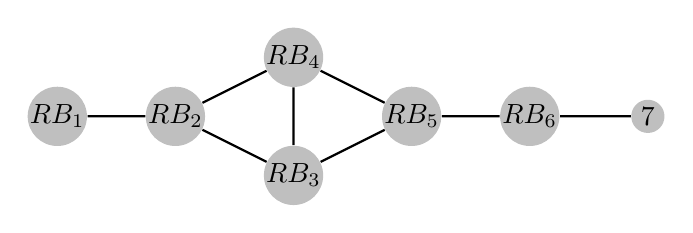
\begin{tikzpicture}[scale=1.5]
    % Draw a 7,11 network
    % First we draw the vertices
    \foreach \pos/\name in {{(1,2)/RB_1}, {(2,2)/RB_2}, {(3,1.5)/RB_3}, {(3,2.5)/RB_4}, {(4,2)/RB_5}, {(5,2)/RB_6}, {(6,2)/7}}
        \node[vertex] (\name) at \pos {$\name$};
    
    
    % Connect vertices with edges 
    \foreach \source/ \dest in {RB_1/RB_2, RB_2/RB_3,RB_2/RB_4,RB_3/RB_5, RB_4/RB_5, RB_5/RB_6, 7/RB_6, RB_4/RB_3}
        \path[edge] (\source) -- (\dest) ;
        
\end{tikzpicture}
\end{center}

\end{example}

Indeed, this monitoring technique will be less invalid if the network is not commonly known. In this example, if Rebels has asymmetric information about network structure, says Rebel 5 (or Rebel 2,3) does not certain about if there is a link between Rebel 4 and Rebel 2, then Rebel 4 can just pretend that he doesn't know Rebel 2\footnote{However, if there is asymmetric information about network structure, then Example ~\ref{ex_no_free_rider_cycle} is not exactly a free rider problem. Dependent on what asymmetric information is given, Rebel 3 and Rebel 4 then have different incentives in untruthful reporting. Untruthful reporting could be a dominant strategy for Rebel 4 but not necessary be a dominant strategy for Rebel 3.}. The analysis in incomplete information about network structure is beyond the scope of this paper. Recent paper such as \citep{Galeotti2010} deal with the issues when network is not commonly known.

There is another free rider problem which is harder to deal with. Remind that the implicit technique in my equilibrium construction is that the pivotal Rebels can be identified before the game is played in each reporting period in each block. When the networks has cycles, the selection of pivotal Rebels needs more elaboration. Consider Example ~\ref{ex_free_rider_cycle}.
\begin{example}\label{ex_free_rider_cycle}
Let $k=6$. Suppose the network and $\theta$ is as the following. 

\begin{center}
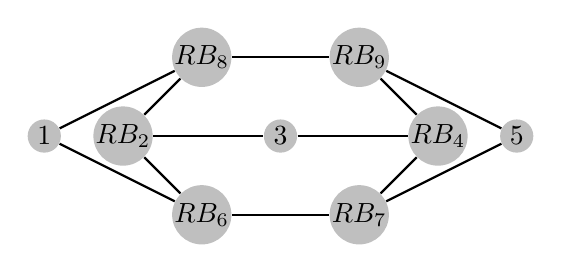
\begin{tikzpicture}[scale=1]
    % Draw a 7,11 network
    % First we draw the vertices
    \foreach \pos/\name in {{(1,3)/1}, {(2,3)/RB_2}, {(4,3)/3}, {(6,3)/RB_4}, {(7,3)/5}, {(3,2)/RB_6}, {(5,2)/RB_7}, {(3,4)/RB_8}, {(5,4)/RB_9}}
        \node[vertex] (\name) at \pos {$\name$};
    
    
    % Connect vertices with edges 
    \foreach \source/ \dest in { 1/RB_6, 1/RB_8, RB_2/3, RB_2/RB_8, 3/RB_4, RB_2/RB_6, RB_6/RB_7, RB_8/RB_9, RB_9/RB_4, RB_7/RB_4, RB_9/5, RB_7/5}
        \path[edge] (\source) -- (\dest) ;
        
\end{tikzpicture}
\end{center}

Assume that one round of reporting is done. Rebel 2 has known $\{RB_2,RB_6,RB_8,RB_9,RB_7\}$, Rebel 4 has known $\{RB_4,RB_7,RB_9,RB_8,RB_6\}$, and so on. One more round of reporting will let Rebels 3,6,7,4,9,8 know the true state $\theta$, and therefore Rebels 3,6,7,4,9,8 are all pivotal players. We may have a rule as Example ~\ref{ex_free_rider_tree} to pick up a pivotal Rebel, say we pick Rebel 4 before entering the next reporting period. However, this pivotal player selection is ex-post. The true state $\theta^{'}$ could be as the following.

\begin{center}
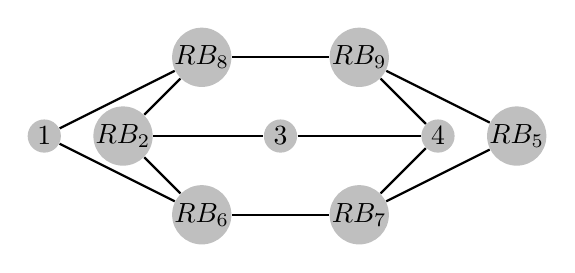
\begin{tikzpicture}[scale=1]
    % Draw a 7,11 network
    % First we draw the vertices
    \foreach \pos/\name in {{(1,3)/1}, {(2,3)/RB_2}, {(4,3)/3}, {(6,3)/4}, {(7,3)/RB_5}, {(3,2)/RB_6}, {(5,2)/RB_7}, {(3,4)/RB_8}, {(5,4)/RB_9}}
        \node[vertex] (\name) at \pos {$\name$};
    
    
    % Connect vertices with edges 
    \foreach \source/ \dest in { 1/RB_6, 1/RB_8, RB_2/3, RB_2/RB_8, 3/4, RB_2/RB_6, RB_6/RB_7, RB_8/RB_9, RB_9/4, RB_7/4, RB_9/RB_5, RB_7/RB_5}
        \path[edge] (\source) -- (\dest) ;
        
\end{tikzpicture}
\end{center}

Now node 4 is an Inert and so that he is not a pivotal Rebel. Some other rules are needed to be applied to select a pivotal Rebel (say, Rebel 5 in this case) during the game is played. 

\end{example}

As Example ~\ref{ex_free_rider_tree} or ~\ref{ex_free_rider_cycle} show, a free rider problem may occur if the selection of pivotal Rebels is not done before the game is played. When the networks has cycles, this problem seems more harsh and the selection rule may not be done before the game is played. Though it is possible to construct a selection rule, this rule is still infeasible in this paper. 

I leave a conjecture here and end this section.

\begin{conjecture}
\label{thm_main_result}
For $n$-person repeated $k$-Threshold game with parameter $1\leq k < n$ played in any FFCCU network,
if the state $\theta$ has strong connectedness and $\pi(\{\theta: \theta\text{ has strong connectedness}\})=1$ with full support, then there is a $\delta$ such that there is a (weak) sequential equilibrium which is APEX.
\end{conjecture}



\section{Conclusion}
\label{sec:con}

I model a coordination game and illustrate the learning processes generated by strategies in a sequential equilibrium and answer the question proposed in the beginning: what kind of networks can conduct coordination in a collective action game with information barrier. In the equilibrium, players transmit the relevant information by encoding such information by their actions in the time horizontal line. Since there is an expected cost in coding information, potential free rider problems may occur to impede the learning process. When the networks are FFCCU without cycle, players can always learn the underlying relevant information and conduct the coordination only by their actions in a equilibrium. However, what kinds of equilibrium strategies can constitute a learning process to learn the relevant information in the networks with cycles still remains to be answered.

Existing literatures in political science and sociology have recognized the importance of social network in influencing individual's behaviour in participating social movements, e.g., \citep{Passy2003}\citep{McAdam2003}\citep{Siegel2009}. This paper views networks as routes for communication where rational individuals initially have local information, and they can influence nearby individuals by taking actions. Such influence may take long time to travel across individuals. A characterization in the speed of information transmission across a network is not answered here, although it is an important topic in order to give more attentions in the details of network structures. This question would remain for the future research.



\bibliographystyle{abbrvnat}	% (uses file "plain.bst")
\bibliography{jmp_ref}		% expects file "myrefs.bib"


\appendix
\section{Appendix}

\noindent\textbf{proof for Lemma ~\ref{lemma_learn}}

\begin{proof}
The proof is done by contradiction. Suppose Rebels' strategies constitute an APEX. By definition of APEX, there is a time $T^{\theta}$ when actions start to repeat at state $\theta$. Let $T=\max_{\theta\in \Theta}{T^{\theta}}$. Pick that time $T_i=T+1$ and suppose the consequence did not not holds so that $0<\sum_{\theta:\#[Rebels](\theta)\geq k}\beta^{\pi,\tau^*}_{G_i}(\theta|h^{s}_{G_i})<1$ for some $s\geq T_i$. Then this Rebel puts some positive weights on some $\theta\in \{\theta:\#[Rebels](\theta)< k\}$ and puts some positive weights on $\theta\in \{\theta:\#[Rebels](\theta)\geq k\}$ at that time $s$. Note this Rebel $i$ has already known $\theta_j$ if $j\in G_i$, and therefore Rebel $i$ put some positive weights on $\theta\in \{\theta:\#[Rebels](\theta)< k, \theta_l=Rebel, l\notin G_i\}$ and $\theta\in \{\theta:\#[Rebels](\theta)< k, \theta_l=Inert, l\notin G_i\}$. Since actions start to repeat at $T$, all $i$'s neighbors will play the same actions as the actions at time $T$, but then Rebel $i$ can not update information from his neighborhood by Bayesian rule. Suppose $i$'s continuation strategy is to play \textbf{revolt} repeatedly, then this is not ex-post efficient if $\#[Rebels](\theta)< k$. Suppose $i$'s continuation strategy is to play \textbf{stay} repeatedly, then this is not ex-post efficient if $\#[Rebels](\theta)\geq k$
\end{proof}

\bigskip
\noindent\textbf{proof for Theorem ~\ref{lemma_empty}}

This proof follows three useful claims, Claim ~\ref{lemma_I_subset_N}, Claim ~\ref{lemma1} and Claim ~\ref{lemma_connected}. First note that $I^t_i$ and $N^t_i$, $t\geq 1$ can be expressed as 
\begin{equation}
\label{eq_info_nb}
I^{t}_i = \bigcup_{k_0\in G_i\cap R^{t}}\bigcup_{k_1\in G_{k_0}\cap R^{t-1}}...\bigcup_{k_{t-1}\in G_{k_{t-2}}\cap R^{1}}G_{k_{t-1}}\cap R^0
\end{equation}
, while $H^t_i$ can be expressed as
\begin{equation}
\label{eq_nb}
N^t_i = \bigcup_{k_0\in G_i\cap R^{t-1}}\bigcup_{k_1\in G_{k_0}\cap R^{t-2}}...\bigcup_{k_{t-2}\in G_{k_{t-3}}\cap R^{0}}G_{k_{t-2}}
\end{equation}

\begin{claim}
\label{lemma_I_subset_N}
$I^t_i\subset N^t_i$ for $t\geq 1$
\end{claim}
\begin{proof}
$I^t_0\subset N^t_0$ by definition. Since $R^t\subset R^{t-1}$ for $t\geq 1$, $I^t_i\subset N^t_i$ for $t\geq 1$ by comparing Equation ~\ref{eq_info_nb} and Equation ~\ref{eq_nb}.
\end{proof}

\begin{claim}
\label{lemma1}
If the network is FFCCU without cycle, then for each $t\geq 1$ block, we have $i\in R^t\Leftrightarrow i\in R^{t-1} \text{ and } \exists k_1,k_2\in R^{t-1}\cap \bar{G}_i$, where $k_1\neq k_2$.
\end{claim}
\begin{proof}
The proof is by induction. We first show that the statement is true for $t=1$. 

\textbf{Base}: $i\in R^1\Leftrightarrow [i\in R^0] \wedge [\exists k_1,k_2\in (R^0\cap \bar{G}_i)]$. 

$\Rightarrow$: Since $i\in R^1$, then $i\in R^0$ and then $I^0_i\nsubseteq N^0_j$ for all $j\in \bar{G}_i$ by definition. Since $I^0_i=R^0\cap G_i$, then $\forall j\in \bar{G}_i [\exists k\in (R^0\cap \bar{G}_i) [k\notin N^0_j]]$. Since the $j\in \bar{G}_i$ is arbitrary,  we then have a pair of $k_1, k_2 \in (R^0\cap \bar{G}_i)$ such that $k_1\notin N^0_{k_2}$ and $k_2\notin N^0_{k_1}$.

$\Leftarrow$: Pick $k\in \{k_1,k_2\}\subseteq (R^0\cap \bar{G}_i)$, and pick an arbitrary $j\in \bar{G}_i\backslash \{k\}$. Note that $k\notin N^0_j$, otherwise there is a cycle from $i$ to $i$. Hence $[k\in (R^0\cap \bar{G}_i)] \wedge [k\notin N^0_j]$ and therefore $[k\in I^0_i] \wedge [k\notin N^0_j]$. Then we have $I^0_i\nsubseteq N^0_j$ for arbitrary $j\in \bar{G}_i$, and thus $i\in R^1$.

\textbf{Induction hypothesis}: the statement is true for $\{1,2,..,t\}$ where $t\geq 1$. 


If the hypothesis is true, then $i\in R^{t+1}\Leftrightarrow [i\in R^{t}] \wedge [\exists k_1,k_2\in (R^{t}\cap \bar{G}_i)]$


$\Rightarrow$: since $i\in R^{t+1}$, then $i\in R^t$ and $I^t_i\nsubseteq N^t_j$ for all $j\in \bar{G}_i$ by definition. Recall that $I^t_i$ can be expressed as Equation ~\ref{eq_info_nb} and $H^t_i$ can be expressed as Equation ~\ref{eq_nb}, then for every $l\in I^{t-1}_i$, we can find a path connecting $i$ to $l$ by the induction hypothesis. If $j\in \bar{G}_i$, then we can find a path connecting $j$ to $l$ by connecting $j$ to $i$, and then connecting $i$ to $l$. Thus, if $l\in I^{t-1}_i$ then $l\in N^t_J$, and hence $I^{t-1}_i\subseteq N^t_{j}$ for all $j\in \bar{G}_i$. Recall that $I^t_i = \bigcup_{k\in N_i\cap R^t}I^{t-1}_k$ and $i\in R^{t+1}$, then we must have $\forall j\in \bar{G}_i [\exists k\in (R^t\cap \bar{G}_i)[ I^{t-1}_k\nsubseteq N^t_j]]$, since $I^{t-1}_i\subseteq N^t_{j}$. Note that such $j\in \bar{G}_i$ is arbitrary,  we then have a pair of $k_1, k_2 \in (R^{t}\cap \bar{G}_i)$ such that $k_1\notin N^t_{k_2}$ and $k_2\notin N^t_{k_1}$.
\bigskip

$\Leftarrow$:
By the induction hypothesis, we have a chain $k_{1_0},...,k_{1_t},i,k_{2_t},...,k_{2_0}$ with $k_{1_0}\in R^0$,..., $k_{1_t}\in R^t$, $i\in R^t$, $k_{2_t}\in R^t$,...,$k_{1_0}\in R^0$, where $k_{1_t},k_{2_t}\in (R^{t}\cap \bar{G}_i)$, $k_{1_0}\in I^{t-1}_{k_{1_t}}$ and $k_{2_0}\in I^{t-1}_{k_{2_t}}$. Note that $k_{1_0}\notin N^t_j$ whenever $j\in \bar{G}_i$, otherwise there is a cycle from $i$ to $i$ since $\{i,k_{2_t},...,k_{2_0}\}\in N^t_j$, and hence $[k_{1_0}\in I^{t-1}_{k_{1_t}}] \wedge [k_{1_0}\notin N^t_j]$ for all $j\in \bar{G}_i$. Therefore we have $[I^{t-1}_{k_{1_t}}\in I^t_i] \wedge [I^{t-1}_{k_{1_t}}\notin N^t_j]$ for all $j\in \bar{G}_i$ since $k_{1_t},k_{2_t}\in (R^{t}\cap \bar{G}_i)$ and $[k_{1_0}\in I^{t-1}_{k_{1_t}}] \wedge [k_{1_0}\notin N^t_j]$ for all $j\in \bar{G}_i$. Then we have $I^t_i=\bigcup_{k\in N_i\cap R^{t}}I^{t-1}_k\nsubseteq N^t_j$ for arbitrary $j\in \bar{G}_i$, and thus $i\in R^{t+1}$.



We can then conclude that the statement is true by induction.




\end{proof}



\begin{claim}
\label{lemma_connected}
If the network FFCCU without cycle and if the state has strong connectedness, then if there is a pair of $R^{t}$ nodes then there exists a $R^{t}$-path connecting them.
\end{claim}
\begin{proof}
The proof is by induction and by Claim ~\ref{lemma1}. Since the state has strong connectedness, we have a $R^0$-path connecting each pair of $R^0$ nodes. Since all pairs of $R^0$ nodes are connected by a $R^0$-path, then for all pairs of $R^1$ nodes must be in some of such paths by Claim ~\ref{lemma1}, and then connected by a $R^0$-path. But then all the $R^0$-nodes in such path are all $R^1$ nodes by Claim ~\ref{lemma1} again and by $R^t\subseteq R^{t-1}$ for $t\geq 1$ by definition. Thus, for all pairs of $R^1$ nodes has a $R^1$-path connecting them. The similar argument holds for $t> 1$, we then get the result.

\end{proof}
I begin to prove this Theorem ~\ref{lemma_empty}. I first claim that if $R^t\neq \emptyset$ and if $R^{t+1}= \emptyset$, then $R^0\subset I^t_i$ whenever $i\in R^t$. Then I claim that if $R^t\neq \emptyset$ then $\# R^{t+1}<\# R^t$. Finally, I iterate $R^t$ with $t\geq 0$ to get the conclusion.

If $R^t\neq \emptyset$ but $R^{t+1}= \emptyset$, I claim that $R^0\subset I^{t}_i$ for all $i\in R^t$. The proof is by contradiction. If $R^0\not\subset I^{t}_i$, there is a $j\in R^0$ but $j\notin I^t_i$. Since $I^t_i$ can be expressed as Equation ~\ref{eq_info_nb}, there is no such a path $\{i,k_0,k_1,...,k_{t-1},j\}$, where $k_0\in G_i\cap R^{t},k_1\in G_{k_0}\cap R^{t-1},...,k_{t-1}\in N_{k_{t-2}}\cap R^{1}$. Since $R^{t+1}=\emptyset$ and therefore $R^{t^{'}}=\emptyset$ if $t^{'}\geq t+1$, and hence there is no such a path containing a node in $R^{t^{'}}=\emptyset$, where $t^{'}\geq t+1$ connecting $i$ to $j$. But $i\in R^t$ and $i,j\in R^0$, if there is no such a path, then it violate either Claim ~\ref{lemma_connected} or Claim ~\ref{lemma1}. Contradiction.

Next I claim that if $R^t\neq \emptyset$ then $\# R^{t+1}<\# R^t$. The proof is the followings. Given a node $i$ in $R^t$, let $j\in R^t$ (could be $i$ itself) be the node connected with $i$ with the maximum shortest $R^t$ path. This $j$ can be found since $R^t\neq \emptyset$ and the network is finite. Then there is no $R^t$ node in $j$'s neighborhood other than the nodes in this path. Since the network is without cycle, there is at most one $R^t$ node in $j$'s neighborhood. But then $j\notin R^{t+1}$ since it violate Claim ~\ref{lemma1}.

Starting from $R^0\neq \emptyset$ and iterating $R^t$ with $t\geq 0$, if $R^t\neq \emptyset$ but $R^{t+1}= \emptyset$, then there is some $i$ with $R^0\subset I^t_i$ as the above paragraph shows; if $R^t\neq \emptyset$ and $R^{t+1}\neq \emptyset$, then we starting from $R^{t+1}$ and iterating $R^{t+1}$ with $t\geq t+1$. Since $\#R^{t+1}<\#R^t$ as the above paragraph shows, there is a time $t^{*}$ with $R^{t^{*}}=\emptyset$, then we get the conclusion.


\bigskip




\noindent\textbf{proof for Lemma ~\ref{lemma_at_most_two_nodes}}

\begin{proof}
Denote $(i,j)$-path as the set of paths from $i$ to $j$. The proof is by contradiction. Suppose there are three or more $R^t$-nodes in $C^t$, then pick any three nodes of them, and denote them as $i_1,i_2,i_3$. Let's say $i_2$ is in a $(i_1,i_3)$-path by strong connectedness, and therefore $i_2\in Tr_{i_1i_2}$ and $i_3\in Tr_{i_2i_3}$. First we show that $i_1\in G_{i_2}$ (or $i_3\in G_{i_2}$). Suppose $i_1\notin N_{i_2}$, since $i_1,i_2\in R^t$, then the $(i_1,i_2)$-path is a $R^t$-path by Claim ~\ref{lemma1}. Let this $(i_1i_2)$-path be $\{i_1,j_1,...,j_n,i_2\}$. Since $i_1,j_1,...,j_n,i_2\in R^t$, we then have $I^{t-1}_{i_1}\nsubseteq N^{t-1}_{j_1},...,I^{t-1}_{j_n}\nsubseteq N^{t-1}_{i_2}$ and $I^{t-1}_{j_1}\nsubseteq N^{t-1}_{i_1},...,I^{t-1}_{i_2}\nsubseteq N^{t-1}_{j_n}$. Since $I^{t-1}_{i_1}\subseteq N^{t-1}_{i_1},...,I^{t-1}_{i_2}\subseteq N^{t-1}_{i_2}$ by Claim ~\ref{lemma_I_subset_N}, we further have $\exists k_1\in R^0[k_1\in N^{t-1}_{j_1}\backslash I^{t-1}_{i_1}]$,...,$\exists k_n\in R^0[k_n\in N^{t-1}_{j_n}\backslash I^{t-1}_{i_2}]$. Since the state has strong connectedness, there is a $R^0$ path connecting $k_1,...,k_n$ by Claim ~\ref{lemma_connected}. But then we have already found $k_1,k_2$ such that $k_1\in N^{t-1}_{j_1}\backslash I^{t-1}_{i_1}$ and $k_2\in \bar{G}_{k_1}$. It is a contradiction that $i_1\in C$.

Now, $i_1,i_2,i_3$ will form a $R^t$-path as $\{i_1,i_2,i_3\}$. With the same argument as the above, we then have $\exists k_1\in R^0[k_1\in N^{t-1}_{i_2}\backslash I^{t-1}_{i_1}]$ and $\exists k_2\in R^0[k_2\in N^{t-1}_{i_3}\backslash I^{t-1}_{i_2}]$, and thus $i_1$ is not in $C$.
\end{proof}


\noindent\textbf{proof for Lemma ~\ref{lemma_no_node_outside}}
\begin{proof}
The proof is by contradiction. Since $i\in R^t$, there is a $j\in (R^{t-1}\cap \bar{G}_i)$ by Lemma ~\ref{lemma1}. Note that $N^{t-1}_j\subseteq \bigcup_{k\in N^{t-1}_i}N_k$ since $N^{t-1}_j =\bigcup_{k\in I^{t-2}_j}N_k$, and $I^{t-2}_j\subseteq I^{t-1}_i\subseteq N^{t-1}_i$. If there is another node outside $\bigcup_{k\in N^{t-1}_i}N_k$ in $Tr_{ij}$, then there must be another node such that there is a path connected to some nodes in $N^{t-1}_j$ since the network is connected. It is a contradiction that $i\in C$.

\end{proof}

\subsection{Equilibrium}
\label{Apn_equilibrium}
\subsubsection{Out-off-path belief}

If Rebel $i$ detects a deviation at $m$ period, he form the belief as
\begin{equation}
\beta_{i}(\{\theta:\theta\in \times_{j\in G_i}\{\theta_j\}\times\{Inert\}^{n-\#G_i}\}|h^{m^{'}}_{G_i})=1 \text{ , } m^{'}\geq m
\end{equation}



\subsubsection{Equilibrium Path: Notations}


\begin{itemize}

\item $\langle \rangle_r$ be the set of finite sequences of actions in which the action \textbf{r} occurs once and only once.
\item $PF(\langle \rangle,m)$ be the $m$-periods prefix of $\langle \rangle$.
\item $(i,j)$-path be the set of paths from $i$ to $j$.

\end{itemize}

\subsubsection{Equilibrium Path: reporting period}

\paragraph{reporting period: notations}
\begin{itemize}
\item $m$ be a period in reporting period in $t$ block.
\item $|\langle RP^t \rangle|$ be the total periods in reporting period in $t$-block
\item $O^{m,t}_i$ be the set of $i$'s neighbors $j$s who has played a sequence $M$ such that $M=PF(\langle I^{t-1}_j \rangle,m)$ and $M \in \langle \rangle_r$ at $m$ period. 
\item $I^{m,t}_i\equiv (\bigcup_{k\in O^{m,t}_i} I^{t-1}_k)\cup I^{t-1}_i$ be the updated relevant information gathered by $i$ at period $m$. Note that $I^{0,t}_i=I^{t-1}_i$ and $I^{|\langle RP^t \langle|,t }_i=I^{t}_i$.
\item $N^{m,t}_i\equiv (\bigcup_{k\in O^{m,t}_i} N^{t-1}_k)\cup N^{t-1}_i$
be the updated neighborhood which contains $I^{m,t}_i$

\item Let 
\[Ex_{I^{m,t}_i}\equiv \{l\notin N^{m,t}_i|\exists l^{'}\in I^{m,t}_i\text{ such that there exists a $(l,l^{'})$-path}\}\]
be all the possible Rebel nodes outside of $N^{m,t}_i$ given $I^{m,t}_i$
\item Let
\[Tr_{I^{m,t}_ij}\equiv Tr_{ij}\cap (Ex_{I^{m,t}_i}\cup I^{m,t}_i)\]
be all the possible Rebel nodes in the $Tr_{ij}$ given $I^{m,t}_i$. 
\end{itemize}
\paragraph{reporting period: automata}
\subparagraph{$i\notin R^{t}$}




\begin{itemize}
\item \textbf{WHILE LOOP}
\begin{itemize}
\item At $m\geq 0$, if $\#Ex_{I^{m,t}_i}\cup I^{m,t}_i< k$, report $\langle \textbf{stay} \rangle$ and then play \textbf{stay} forever.
\item Otherwise, \textbf{runs POST-CHECK }
\end{itemize}
\end{itemize}

\subparagraph{$i\in R^{t}$}

\begin{itemize}

\item \textbf{WHILE LOOP}
\begin{itemize}
\item At $m\geq 0$, if $\# Ex_{I^{m,t}_i}\cup I^{m,t}_i< k$, report $\langle \textbf{stay} \rangle$ and then play \textbf{stay} forever.
\item Otherwise, \textbf{runs MAIN }
\end{itemize}


\item \textbf{MAIN}

At $m\geq 0$, 

\begin{enumerate}
\item At $m=0$ and if $\# I^{t-1}_i=\# I^{0,t}_i= k-1$, then 
\textbf{runs POST-CHECK }


\item At $m=0$ and if $i\in R^t$ and
\[\nexists j\in R^{t-1}\cap\bar{G}_i \text{ such that }\exists l_1,l_2\in Tr_{ij}[[l_1\in N^{t-1}_j\backslash I^{t-1}_i] \wedge [l_2\in \bar{G}_{l_1}]]]\]
, then runs \textbf{CHECK.$0$}. Otherwise, recall \textbf{MAIN}
\item At $0\leq m \leq |RP^t|-|\langle I^{t-1}_i \rangle|$, play
\[\textbf{stay}\]
\item At $m = |RP^t|-|\langle I^{t-1}_i \rangle|+1$, then
\begin{enumerate}
\item if $O^{m,t}_i= \emptyset$ 
, then report
\[\langle I^{t-1}_i \rangle\]
\item if $O^{m,t}_i\neq \emptyset$, then \textbf{runs CHECK.k}

\end{enumerate}

\end{enumerate}





\item \textbf{CHECK.$0$}

At $m=0$, if $i\in C^t$, i.e. if $i\in R^t$ and
\[\nexists j\in R^{t-1}\cap \bar{G}_i \text{ such that }[\exists l_1,l_2\in Tr_{ij}[[l_1\in N^{t-1}_j\setminus I^{t-1}_i] \wedge [l_2\in \bar{G}_{l_1}]]]\]
, then
\begin{enumerate}
\item If $\#C^t=1$
, then 
\textbf{runs POST-CHECK }

\item If $\#C^t=2$, then denote $i_1,i_2\in C$ such that $I^{t-2}_{i_1}<I^{t-2}_{i_2}$, and then
\begin{itemize}
\item if $i=i_1$, then 
\textbf{runs POST-CHECK }
\item if $i=i_2$, then report
\[\langle I^{t-1}_i \rangle\]

\end{itemize}
\end{enumerate}




\item \textbf{CHECK.$m$}

 At $m>0$, if $O^{m,t}_i\neq \emptyset$, then there are two cases, 
\begin{enumerate}
\item Case 1: If $i\in R^t$ and 
\[\exists j\in  O^m_i \text{ such that }\exists l_1,l_2\in Tr_{I^{m,t}_ij}[[l_1\in I^{t-1}_j\backslash I^{t-1}_i] \wedge [l_2\in \bar{G}_{l_1}]]]\]
, then report 
\[\langle I^{t-1}_i \rangle\]
\item Case 2: If $i\in R^t$ and 
\[\not\exists j\in  O^m_i \text{ such that }\exists l_1,l_2\in Tr_{I^{m,t}_ij}[[l_1\in I^{t-1}_j\backslash I^{t-1}_i] \wedge [l_2\in \bar{G}_{l_1}]]]\]

\begin{enumerate}
\item Case 2.1: If $i\in R^t$ and 
\[\not\exists j\in R^{t-1}\cap (G_i\backslash  O^{m,t}_i) \text{ such that }[\exists l_1,l_2\in Tr_{I^{m,t}_ij}[[l_1\in N^{t-1}_j\backslash I^{t-1}_i] \wedge [l_2\in \bar{G}_{l_2}]]]\]
\[\textbf{Note: this case is the case when $i\in C$, thus recall Check.0}\]

\item Case 2.2: If $i\in R^t$ and 
\[\exists j\in R^{t-1}\cap (G_i\backslash  O^{m,t}_i) \text{ such that }[\exists l_1,l_2\in Tr_{I^{m,t}_ij}[[l_1\in N^{t-1}_j\backslash I^{t-1}_i] \wedge [l_2\in \bar{G}_{l_2}]]]\]

\begin{itemize}
\item if $\# I^{m,t}_i= k-1$
, then 
\textbf{runs POST-CHECK }

\item if $\# I^{m,t}_i< k-1$
, then report 
\[\langle I^{t-1}_i \rangle\]
\end{itemize}





\end{enumerate}

\end{enumerate}





\item \textbf{CHECK.k}

At $m\geq 1$, 
\begin{enumerate}


\item $O^{m,t}_i\neq \emptyset$, and
 \[\# I^{m,t}_i\geq k\]
, then 
\textbf{runs POST-CHECK }

\item $O^{m,t}_i\neq \emptyset$, and 
\[ \#I^{m,t}_i< k\]
, then \textbf{runs CHECK.$m$}
\end{enumerate}


\item \textbf{POST-CHECK}

\begin{enumerate}


\item At $m=|RP^t|$, then
\begin{enumerate}
\item If $i\in R^t$ and if $|I^{m,t}_i|\geq k-1$, then play
\textbf{revolt}

\item if $i\notin R^t$, then play
\textbf{stay}


\end{enumerate}
\end{enumerate}


\end{itemize}



\subsubsection{Equilibrium path: coordination period}
\paragraph{coordination period: notations}
\begin{itemize}
\item $m$ be a sub-block in coordination period.
\item Let 
\[Ex_{I^{t}_i}\equiv \{l\notin I^{t}_i|\exists l^{'}\in I^{t}_i\setminus I^{t-1}\text{ such that there exists a $(l,l^{'})$-path}\}\]
be all the possible Rebel nodes outside of $N^{t}_i$ given $I^{t}_i$.

\item Let
\[Tr_{I^{t}_ij}\equiv Tr_{ij}\cap (Ex_{I^{t}_i}\cup I^{t}_i)\]
be the set of possible Rebel nodes in the $Tr_{ij}$ given $I^{t}_i$. 

\end{itemize}




\paragraph{coordination period: automata}


\begin{itemize}





\item \textbf{1st Division} 

In 1st division, for $t=0$ block,

\begin{itemize}



\item If $\# Ex_{I^{t}_i}\cup I^{t}_i<k$, then play \textbf{stay} forever.

\item If $\# Ex_{I^{t}_i}\cup I^{t}_i \geq k$, and if $i\not\in R^1$, then play
\[\langle \textbf{stay} \rangle\]

\item If $\# Ex_{I^{t}_i}\cup I^{t}_i \geq k$, and if $i\in R^1$, then play
\[\langle \mathbf{1}_i \rangle\]


\end{itemize}

In 1st division, for $t>0$ block and for $1\leq m \leq n$ sub-block,
\begin{itemize}

\item If $i$ has played $\langle 1 \rangle$, then play 
\[\langle \mathbf{1}_i \rangle\]

\item If $\# Ex_{I^{t}_i}\cup I^{t}_i<k$, then play \textbf{stay} forever.

\item If $\# Ex_{I^{t}_i}\cup I^{t}_i\geq k$, and there are some $j\in \bar{G}_i$ have played $\langle \textbf{stay} \rangle $, then play
\textbf{stay} forever.
\item If $\# Ex_{I^{t}_i}\cup I^{t}_i \geq k$, and there is no $j\in \bar{G}_i$ has played $\langle \textbf{stay} \rangle $, then play
\[\langle \mathbf{1}_i \rangle\]

\end{itemize}




\item \textbf{2nd Division} 

In $t=0$ block
\begin{itemize}
\item If $i\notin R^1$, play \[\langle \textbf{stay} \rangle \].
\item If $i\in R^1$, and if $\#I^0_i\geq k$, play \[\langle \textbf{stay} \rangle \].
\item If $i\in R^1$, if $\#I^0_i< k$, if $\# Ex_{I^{t}_i}\cup I^{t}_i\geq k$ and if some $j\in \bar{G}_i$ have played play $\mathbf{1}_j$ in the 1st division, then play \[\langle \textbf{stay} \rangle \].
\item If $i\in R^1$, if $\#I^0_i< k$, if $\# Ex_{I^{t}_i}\cup I^{t}_i\geq k$ and if no $j\in \bar{G}_i$ has played play $\mathbf{1}_j$ in the 1st division, then play \textbf{stay} forever.

\end{itemize}


In $t>0$ block, if there is no $j\in G_i$ such that $j$ has played $\langle \textbf{stay} \rangle$ in the \textbf{1st Division} , then run the following automata. Otherwise, play \textbf{stay} forever.

\begin{itemize}
\item $i\notin R^t $
\begin{itemize}
\item In the $1$-sub-block: play
\[\langle \textbf{stay} \rangle \]


\item In the $2\leq m\leq t+1$ sub-blocks: 

\begin{enumerate}

\item If $i\in R^{t^{'}}$ for some $t^{'}\geq 0$ and if there is a $j\in R^{t^{'}+1}\cap \bar{G}_i$ has played 
\begin{enumerate}
\item $\langle \textbf{stay} \rangle $ in $m=1$ sub-block
\item or $\langle \mathbf{1}_j \rangle$ in $m\geq 2$ sub-blocks
\end{enumerate}
, then play 
\[\langle \mathbf{1}_i \rangle\] in $m+1$ sub-block.

\item Otherwise, play
\[\langle \textbf{stay} \rangle\] in current sub-block
\end{enumerate}

\end{itemize}

\item $i\in R^t$

\begin{itemize}
\item In the $1$-sub-block:
\begin{enumerate}
\item If $i$ has played $\langle 1 \rangle$, then play
\[\langle \textbf{stay} \rangle \]

\item If $i$ has not played $\langle 1 \rangle$ and if there is a $j\in \bar{G}_i$ has played $\langle 1 \rangle$, then play
\[\langle \textbf{stay} \rangle \]

\item If $i$ has not played $\langle 1 \rangle$ and if there is no $j\in \bar{G}_i$ has played $\langle 1 \rangle$, then
\begin{itemize}
\item If $\# I^{|RP^t|,t}_i\geq k$, then play
\[\langle \textbf{stay} \rangle \]
\item If $\# I^{|RP^t|,t}_i< k$, then play
\[\langle \mathbf{1}_i  \rangle \]
\end{itemize}

\end{enumerate}

\item In the $m\geq 2$-sub-block: 

\begin{enumerate}

\item If $i\in R^{t^{'}}$ for some $t^{'}\geq 0$ and if there is a $j\in R^{t^{'}}\cap \bar{G}_i$ has played 
\begin{enumerate}
\item $\langle \textbf{stay} \rangle$ in $m=1$ sub-block, or
\item $\langle \mathbf{1}_j \rangle$ in $m\geq 2$ sub-blocks
\end{enumerate}
, then play 
\[\langle \mathbf{1}_i \rangle\] in $m+1$ sub-block.
\item Otherwise, play
\[\langle \textbf{stay} \rangle\] in current sub-block.
\end{enumerate}

\end{itemize}

\end{itemize}



\item \textbf{3rd Division} 

\begin{enumerate}
\item \textbf{INITIATING} 

If $i$ has observed $j\in \bar{G}_i$ has played
\begin{enumerate}
\item $\langle \textbf{stay} \rangle$ in $1$-sub-block in \textbf{2nd Division}  or
\item $\langle \mathbf{1}_j \rangle$ in $m\geq 2$ sub-blocks \textbf{2nd Division}  or
\item \textbf{s} in the \textbf{3rd Division} 
\end{enumerate}
, then play \textbf{revolt} forever

\item \textbf{NOT INITIATING} 

Otherwise, play 
\textbf{stay} 
in current period.
\end{enumerate}
\end{itemize}





\subsubsection{Proof for Theorem ~\ref{thm_main_result}}


The proof is organized as the following. In Claim ~\ref{claim_either_success_or_fail} and Lemma ~\ref{lemma_in_the_path}, we show that a Rebel will learn $\#[Rebels](\theta)\geq k$ or $\#[Rebels](\theta)< k$ in the equilibrium path. Lemma ~\ref{lemma_in_the_path} also show that the equilibrium path is ex-post efficient. Since that, there is a time $T$ such that a Rebel's static pay-off after $T$ is $1$ if $\#[Rebels](\theta)\geq k$ or $0$ if $\#[Rebels](\theta)\geq k$. Such pay-offs after time $T$ is the maximum static pay-off contingent on $\theta$. In Claim ~\ref{claim_detection_reporting_period}, I show that if a Rebel makes detectable deviation, then there is a positive probability event $E$ (by the full support assumption) contingent on this deviation such that his expected continuation static pay-off is strictly lower than that in equilibrium path after $T$. Finally, in Claim ~\ref{claim_deviation_higher_reporting}, Claim ~\ref{claim_can_not_pretend_almost_success}, Claim ~\ref{claim_must_report_1}, and Claim ~\ref{claim_report_with_no_message_coordination_period}, I show that if a Rebel makes undetectable deviation, then there is a positive event $E$ (by the full support assumption) contingent on this deviation such that his expected continuation static pay-off is also strictly lower than that in equilibrium path after $T$. Since the static pay-off after $T$ is maximum for all $\theta$ in equilibrium path, there is a $\delta$ such that a Rebel will not deviate. I then conclude this theorem.

To simplify the notations, if $P(\theta)$ is a property of $\theta$, then I abuse the notations by letting $\beta^{\pi,\tau^*}_{G_i}(P(\theta)|h^{m}_{G_i})\equiv \sum_{\theta:P(\theta)}\beta^{\pi,\tau^*}_{G_i}(\theta|h^{m}_{G_i})$. I also say ``$i$ knows $P(\theta)$'' to mean $\beta^{\pi,\tau^*}_{G_i}(P(\theta)|h^{m}_{G_i})=1$. 




\begin{claim}
\label{claim_either_success_or_fail}
In the equilibrium path and for $\#Ex_{I^{m,t}_i}\cup I^{m,t}_i\geq k$, where $m$ is a period in reporting period. If $i$ report $\langle 1 \rangle$, then either Rebels coordinate to \textbf{revolt} after $t$-block or $\# R^0<k$.
\end{claim}
\begin{proof}
By directly checking the equilibrium path, we have
\begin{enumerate}
\item if $\# I^{|RP^t|,t}_i\geq k$, then the coordination can be initiated by such $i$.
\item if $\# I^{|RP^t|,t}_i= k-1$, and if there is one more node who reported $\langle 1 \rangle$, then the coordination can be initiated by $i$.
\item if $\# I^{|RP^t|,t}_i= k-1$, and if there are no nodes who reported in current reporting period, then $\# I^{|RP^t|,t}_i=\# I^{t}_i= k-1$. We now check the conditions guiding $i$ to \textbf{POST-CHECK}.
\begin{itemize}
\item If $i$ is coming from the conditions in \textbf{MAIN}, it means that there are no further Rebels outside $I^{t-1}_i$, thus outside $\bigcup_{k\in I^{t-1}_i}G_k$.
\item If $i$ is coming from the conditions in \textbf{CHECK.0}, it means that there are no further Rebels outside $\bigcup_{k\in I^{t-1}_i}G_k\cap R^0$, and thus outside $\bigcup_{k\in I^{t-1}_i}G_k$. 
\item If $i$ is coming from the conditions in \textbf{CHECK.m}, it means that there are no further Rebels outside $\bigcup_{k\in I^{t-1}_i}G_k\cap R^0$, and thus outside $\bigcup_{k\in I^{t-1}_i}G_k$. 
\end{itemize}
Since $I^t_i=\bigcup_{k\in I^{t-1}_i}G_k\cap R^0 \subset \bigcup_{k\in I^{t-1}_i}G_k$ and $\#I^t_i<k$, and hence $\# R^0<k$.

\end{enumerate}


\end{proof}




\noindent \textbf{proof for Lemma ~\ref{lemma_in_the_path}}
\begin{proof}
We want to show that when $\theta$ satisfying $\#[Rebels](\theta)\geq k$, all the Rebels play \textbf{revolt} eventually; when $\theta$ satisfying $\#[Rebels](\theta)< k$, all the Rebels play \textbf{stay} eventually.
\begin{enumerate}
\item If all the Rebels only play $\langle I^{t-1} \rangle$ or $\langle \textbf{stay} \rangle$ in reporting period for all $t\geq 1$ block, then by the equilibrium path, those nodes played $\langle I^{t-1} \rangle$ are $R^t$-node, and those nodes played $\langle \textbf{stay} \rangle$ are non-$R^t$ nodes. 

If there are some Rebels play $\langle \textbf{stay} \rangle$ in $CD^t_{1,1}$, then all the Rebels play \textbf{stay} eventually; If $R^t$ Rebels play $\langle \textbf{stay} \rangle$ in $CD^t_{1,2}$, then all the Rebels will play \textbf{revolt} after third division in coordination period in this block. Otherwise, all the Rebels go to the next reporting period.

By Theorem ~\ref{lemma_empty}, there is a $t^{*}$ such that there is a $R^{t^{*}}$ node knows $\theta$, and therefore he knows if $\theta$ satisfying $\#[Rebels](\theta)\geq k$ or $\#[Rebels](\theta)< k$. In equilibrium path, such node play $\langle \textbf{stay} \rangle$ either in $CD^{t^{*}}_{1,1}$ or in $CD^{t^{*}}_{1,2}$. Thus the equilibrium path is APEX.

\item If there are some Rebels play $\langle 1 \rangle$ in reporting period for a $t\geq 1$ block, then by Claim ~\ref{claim_either_success_or_fail}, such nodes will knows if $\theta$ satisfying $\#[Rebels](\theta)\geq k$ or $\#[Rebels](\theta)< k$ after reporting period in this $t$-block. Then $\langle \textbf{stay} \rangle$ is either played in the first sub-block in first division or played in the first sub-block in second division in coordination period. Thus the equilibrium path is APEX.

 
\end{enumerate}

\end{proof}



Next, I prepare the claims to show that a Rebel will not deviate. I start with Claim ~\ref{claim_detection_reporting_period} in which the deviation is detectable.


\begin{claim} 
\label{claim_detection_reporting_period}
For $\#Ex_{I^{m,t}_i}\cup I^{m,t}_i\geq k$, where $m$ is a period. Denote $D$ be the set of Rebels who detect $i$'s deviation. If $\# I^{m,t}_i<k$ and if $D\neq \emptyset$, then there is a $\delta$ such that $i$ will not deviate.
\end{claim}
\begin{proof}

Denote $D$ be the set of neighbors who detect $i$'s deviation. Let the events be
\begin{eqnarray*}
E_1 	&= &\{\theta: \#[Rebels](\theta)< k\}\\
E_2 	&= &\{\theta: k\leq \#[Rebels](\theta)<k+\# D\}\\
E_3 	&= &\{\theta: \#[Rebels](\theta)\geq k+\# D\}
\end{eqnarray*}

In equilibrium path, there are periods $t^{s}$ ($t^{f}$) such that if $\theta$ satisfying $\#[\text{Rebels}](\theta)\geq k$ ( $\#[\text{Rebels}](\theta)< k$) then Rebels play \textbf{revolt} (\textbf{stay}) forever. If $i$ follows the equilibrium path, the expected static pay-off after $\max\{t^s,t^f\}$\footnote{There is $t^{s}$ or $t^{f}$ for each $\theta$. The maximum is among those possible $\theta$.} is
 \[\beta_{i}(E_2|h^{m}_{N_i})+\beta_{i}(E_3|h^{m}_{N_i})\]

If $i$ deviate, the expected static pay-off after $\max\{t^s,t^f\}$ is
 \[\beta_{i}(E_3|h^{m}_{N_i})\]
 
Therefore there is a loss in expected static pay-off of
\[\beta_{i}(E_2|h^{m}_{N_i})\]

Thus, there is a loss in expected continuation pay-off contingent on $E_2$ by
\[\delta^{\max\{t^s,t^f\}}\frac{\beta_{i}(E_2|h^{m}_{N_i})}{1-\delta}\]

Note that $\beta_{i}(E_2|h^{m}_{N_i})>0$, since $\#Ex_{I^{m,t}_i}\cup I^{m,t}_i\geq k$ and therefore $\beta_{i}(\#[Rebels](\theta)\geq k|h^{m}_{N_i})>0$ by full support assumption.
\end{proof}


Next, I prepare the claims to show that a Rebel will not deviate if such deviation is undetectable.

\begin{claim} 
\label{claim_deviation_higher_reporting}
In reporting period for $\# Ex_{I^{m,t}_i}\cup I^{m,t}_i \geq k$, if $\# I^{m,t}_i<k$, then there is a $\delta$ such that $i$ will not deviate by reporting $\bar{I}^{t-1}_i\neq I^{t-1}_i$ if such deviation is not detected by $i$'s neighbor.
\end{claim}

\begin{proof}
Assume $\bar{I}^{t-1}_i\neq I^{t-1}_i$. Since a detection of deviation has not occur, it must be the case that there is a non-empty set $F=\{j\in \bar{I}^{t-1}_i:\theta_j=Inerts\}$\footnote{Otherwise, there is a detection of deviation. Recall the definition in information hierarchy: $I^{-1}_i\subset I^{0}_i\subset...\subset I^{t-1}_i$ for all $i\in R^0$}. 


Let the set 
\[E_1=\{\bar{\theta}: \bar{\theta}_j=Rebel \text{ if } j\in F \text { and }\bar{\theta}_j=\theta_j \text{ if } j\notin F\}\]
be the set of pseudo events by changing $\theta_j$ where $j\in F$. And let
\[E_2=\{\theta: \theta_j=Inert \text{ if }j\in F \text { and }\bar{\theta}_j=\theta_j \text{ if } j\notin F\}\]
be the set of true event.

Then consider the event
\begin{eqnarray*}
E 	&= &\{\bar{\theta}\in E_1: \#[Rebels](\bar{\theta})\geq k\}\\
 	&= &\{\theta\in E_2: \#[Rebels](\theta)\geq k-\#F\}
\end{eqnarray*}

Partition $E$ as sub events
\begin{eqnarray*}
E_3 	&= &\{\theta\in E_2: \#[Rebels](\theta)\geq k\}\\
E_4 	&= &\{\theta\in E_2: k>\#[Rebels](\theta)\geq k-\#F\}
\end{eqnarray*}

By Lemma ~\ref{lemma_empty} and following the strategies in equilibrium path (since $i$ have not been detected), there is a block $\bar{t}^{s}$ with respect to $\bar{\theta}$ such that if $\bar{\theta}\in E$ then there some $R^{\bar{t}^s}$ Rebel $j$s, says $J$, will initiate the coordination, and then Rebels play \textbf{revolt} forever after $\bar{t}^s$-block. Note that such $j$ is with $\# {I}^{\bar{t}^{s}}_i \geq k$ by checking the equilibrium path.

We have several cases:
\begin{enumerate}
\item Case 1: If $i\in J$, his own initiation will only depends on $\# I^{\bar{t}^s}_i$ by Claim ~\ref{claim_can_not_pretend_almost_success} and Claim ~\ref{claim_must_report_1}, which is the same as he has reported $\langle {I}^{t-1}_i\rangle$. He is strictly better off by not deviating since playing $\langle\bar{I}^{t-1}_i\rangle$ is more costly than $\langle\bar{I}^{t-1}_i\rangle$ (since $X_{\bar{I}^{t-1}_i}>X_{I^{t-1}_i}$).

\item Case 2: If there is another $j$ such that $\bar{I}^{t-1}_i\not\subset I^{\bar{t}^{s}}_j$, then since such $j$'s initiation of coordination dependent on his own information $I^{\bar{t}^{s}}_j$ by Claim ~\ref{claim_can_not_pretend_almost_success} and Claim ~\ref{claim_must_report_1}, and $i$'s deviation did not change $j$'s information. It is strictly better by not deviating since playing $\langle\bar{I}^{t-1}_i\rangle$ is more costly than $\langle\bar{I}^{t-1}_i\rangle$ (since $X_{\bar{I}^{t-1}_i}>X_{I^{t-1}_i}$).

\item Case 3: Suppose there is another $j$ such that $\bar{I}^{t-1}_i\subset {I}^{\bar{t}^{s}}_j$ and $\# I^{\bar{t}^s}_i\geq k$, then such $j$ will initiate  the coordination to \textbf{revolt}. If $i$ did not follow $j$'s initiation of coordination, then there is a detection of deviation by checking the equilibrium path. $i$ will not deviate as Claim ~\ref{claim_detection_reporting_period} shows. If $i$ follows, and $\#I^{\bar{t}^s}_i\geq s$, we are in the Case 1. If $i$ follows, but $\#I^{\bar{t}^s}_i< s$, then $i$'s expected static pay-off after $\bar{t}^{s}$ is at most
\[
{\max\{\beta_{i}(E_3|h^{m}_{N_i})\times 1+\beta_{i}(E_4|h^{m}_{N_i})\times (-1), 0\}}
\]

However, if $i$ follow the equilibrium path, there is are $t^s$, $t^f$ such that the expected static pay-off after $\max\{t^s,t^f\}$ is
\[\max\{\beta_{i}(E_3|h^{m^{'}}_{N_i}),0\}\]

Thus, there is a loss in expected continuation pay-off contingent on $E$ by
\[\delta^{\max\{t^s,t^f\}}\frac{\min\{\beta_{i}(E_3|h^{m}_{G_i}),\beta_{i}(E_4|h^{m}_{G_i})\}}{1-\delta}\]
\end{enumerate}

Note that $\beta_{i}(E_3|h^{m}_{N_i})>0$ and $\beta_{i}(E_3|h^{m}_{N_i})>0$, since $\#Ex_{I^{m,t}_i}\cup I^{m,t}_i\geq k$ and $\# I^{m,t}_i<k$, and therefore $1>\beta_{i}(\#[Rebels](\theta)\geq k|h^{m}_{N_i})>0$ by full support assumption.
\end{proof}



\begin{claim} 
\label{claim_can_not_pretend_almost_success}
In reporting period for $\#Ex_{I^{m,t}_i}\cup I^{m,t}_i\geq k$, if $\#I^{m,t}_i\leq k-1$ and if $i\notin C^t$ or $i$ did not satisfy the condition to play $\langle 1 \rangle$ in equilibrium path, then $i$ will not play $\langle 1 \rangle$.
\end{claim}


\begin{proof}


Let
\[E^{'}=\{\theta:\#I^{RP^t,t}_i\leq k-1\}\]
. Note that such event is not empty by checking the timing where $i$ deviated:
\begin{enumerate}
\item If $i$ has a neighbor $j\in C^t$, then $j\not\in O^{RP^t,t}_i$, and therefore we can construct $E^{'}$ by assuming that all other neighbors (other than $i,j$ and other than $l\in O^{m,t}_i$) are non-$R^t$.
\item If \[\exists j\in R^{t-1}\cap \bar{G}_i \text{ such that } \exists k_1,k_2\in Tr_{ij}[[k_1\in N^{t-1}_j\backslash I^{t-1}_i] \wedge [k_2\in \bar{G}_{k_2}]]\], then just let $E^{'}=\{\theta: N^t_i\cap R^0\leq k-1\}=\{\theta: I^t_i\leq k-1\}$\footnote{note that $I^t_i$=$I^{RP^t,t}_i$}.
\end{enumerate}

Next, let 
\begin{eqnarray*}
E_1&=&\{\theta: \#[Reble](\theta)<k\}\cap E^{'}\\
E_2&=&\{\theta: \#[Reble](\theta)\geq k\}\cap E^{'}\\
\end{eqnarray*}

Note that $E_1$ and $E_2$ are not empty. According to equilibrium path, if $i$ did not follow the conditions to play $\langle 1 \rangle$, it must be the case that there are some nodes outside $I^t_i$ but there is a path consisting of Rebels to connect them. By strong connectedness, $E_1$ and $E_2$ are not empty.

Since $i$ deviate to play $\langle 1 \rangle$, his behavior after $CD^t_{1,1}$ will decide the following three cases:
\begin{enumerate}
\item If $i$ play $\langle \textbf{stay} \rangle$ in $CD^t_{1,1}$, then the coordination to \textbf{stay} starts after $CD^t_{1,1}$.
\item If $i$ play $\langle \mathbf{1}_i \rangle$ in $CD^t_{1,1}$, then the coordination to \textbf{revolt} will be initiate after $CD^t_{1,2}$ if he mimic the behavior of a pivotal player (i.e., by mimicking those players who played $\langle 1 \rangle$ in equilibrium path).
\item If $i$ play $\langle \mathbf{1}_i \rangle$ in $CD^t_{1,1}$, but he did not mimic the behavior of pivotal player, then such deviation will be detected.
\end{enumerate}

Thus, $i$'s expected static pay-off after the coordination period in this $t$-block is at most 
\[
{\max\{\beta_{i}(E_2|h^{m}_{N_i})\times 1+\beta_{i}(E_1|h^{m}_{N_i})\times (-1), 0\}}
\]

However, if he stay in the equilibrium, there is a $t^s$ ($t^f$) such that Rebels play \textbf{revolt} (\textbf{stay}) contingent on $E_2$ ($E_1$), and thus after $t^*=\max\{t^s,t^f\}$ he get the expected pay-off as
\[
{\max\{\beta_{i}(E_2|h^{m}_{N_i})\times 1, 0\}}
\]

After some calculation, after $t^*$, there is a loss of
\[\delta^{t^{*}}\frac{\min\{\beta_{i}(E_2|h^{m}_{G_i}),\beta_{i}(E_1|h^{m}_{G_i})\}}{1-\delta}\]
 



Note that $\beta_{i}(E_1|h^{m}_{N_i})>0$ and $\beta_{i}(E_2|h^{m}_{N_i})>0$, by $E_1$ and $E_2$ are not empty and by full support assumption.


\end{proof}







\begin{claim}
\label{claim_must_report_1}
In reporting period for $\beta_{i}(\#[Rebels](\theta)\geq k|h^{RP^t-1}_{G_i})>0$,  then if $i$ can report $\langle 1 \rangle$, then $i$ will not report $\langle l \rangle$ when $\delta$ is high enough.
\end{claim}

\begin{proof}

There are two cases when $i$ can play $\langle 1 \rangle$.
\begin{itemize}

\item Case 1: If $\#I^{|RP^t|-1,t}_i\geq k$, let the event $E$ be
\[E=\{\theta: \#[Rebels](\theta)=\# I^{|RP^t|,t}_i\}\]

That is, the event that no more Rebels outside $i$'s information about Rebels. Contingent on $E$, there is no more Rebel can initiate the coordination. This is because for all $j\in O^{|RP^t|-1,t}_i$, $j$ is with $\# I^{t-1}_j< k-1$, and for all $j\in \bar{G}_i$ who have not yet reported, $j\not\in R^t$ since all the Rebels are in $I^{|RP^t|-1,t}_i$. Since only $i$ can initiate the coordination, if $i$ deviated, compared to equilibrium, there is a loss in expected continuation pay-off as
\[\delta^q\frac{\beta_{i}(E|h^{m}_{N_i})}{1-\delta}\], where $q$ is a period after $t$-block.

\item Case 2: If $\#I^{|RP^t|-1,t}_i= k-1$, since $\beta_{i}(\#[Rebels](\theta)\geq k|h^{|RP^t|}_{G_i})>0$, the following event $E_1$ must have positive probability; otherwise, since no neighbors can report after current period, and thus $\beta_{i}(\#[Rebels](\theta)\geq k|h^{|RP^t|}_{G_i})=0$.

Let
\[E_1=\{\theta: \exists j\in \bar{G}_i, j\notin O^{|RP^t|-1,t}_i [\#I^{|RP^t|-1,t}_j\geq k-1]\}\]


Let sub-events $E^{'}_1\subset E_1$ as

\[E^{'}_1=\{\theta: \text{ exist a unique} j\in \bar{G}_i, j\notin O^{|RP^t|-1,t}_i [\#I^{|RP^t|-1,t}_j\geq k-1]\}\] 

Note that this $E^{'}_1$ can be constructed since the network is tree. If there is $\theta$ admits 2 or more $j$s in the definition $E_1$, these $j$s are not each others' neighbor. Suppose there are two $j$s, says $j$, $j^{'}$, there must be at least one node in $I^{|RP^t|-1,t}_j$ but outside of $I^{|RP^t|-1,t}_{j^{'}}$. We then pick a $j$, and suppose those nodes outside $I^{|RP^t|-1,t}_j$ are all Inerts.

Now, dependent on such $j$, let
\[E=\{\theta:\#[Rebels](\theta)=\#I^{|RP^t|-1,t}_j\cup I^{|RP^t|-1,t}_i\}\]

If $i$ report $\langle l \rangle$, there are following consequences.

\begin{itemize}
\item $i$ will be consider as $\notin R^t$ by $j$, and thus $i$ can not initiate the coordination.
\item Such $j$ has $\#I^{|RP^t|,t}_j=\#I^t_j<k$. Since there is no more Rebel outside $I^{|RP^t|-1,t}_j\cup I^{|RP^t|-1,t}_i$ contingent on $E$, such $j$ will then play \text{stay} forever after $t$-block.
\item Without such extra Rebels in $I^{|RP^t|,t}_j$, only $\#I^{|RP^t|-1,t}_i= k-1$ Rebels may play \textbf{revolt}, and therefore there is no coordination to \textbf{revolt}
\end{itemize}

However, if $i$ play $\langle 1 \rangle$, coordination can be initiated by himself in the following coordination period. Thus, there is a loss in expected continuation pay-off by
\[\delta^{q}\frac{\beta_{i}(E|h^{m}_{N_i})}{1-\delta} \], where $q$ is a period after $t$-block.
\end{itemize}

\end{proof}




\begin{claim} 
\label{claim_report_with_no_message_coordination_period}
Given a $m$ period in coordination period in $t$-block, suppose there is no $j\in G_i$ has played $\langle 1 \rangle$ in reporting period in $t$-block, suppose $\# I^t_i<k$, and suppose $\# Ex_{I^{t}_i}\cup I^{t}_i \geq k$, then there is $\delta$ such that 
\begin{itemize}
\item if $i$ has not observed $\langle \textbf{stay} \rangle$ played by $j\in G_i$ in $CD^t_{1,2}$, or
\item if $i$ has not observed $\langle \mathbf{1}_j \rangle$ played by $j\in G_i$ in $CD^t_{q,2}$, $g\geq 2$
\end{itemize}
, then $i$ will not play
\begin{itemize}
\item $\langle \textbf{stay} \rangle$  in $CD^t_{1,2}$ and
\item $\langle \mathbf{1}_j \rangle$  in $CD^t_{q+1,2}$, $g\geq 2$
\end{itemize}
\end{claim}

\begin{proof}


If $i$ deviate, all $i$'s neighbor who did not detect the deviation will play $\textbf{revolt}$ after coordination period in this block; if $i$'s deviation is detected by some neighbors, we are in the case of Claim ~\ref{claim_detection_reporting_period} and so that $i$ will not deviate. We then check if $i$ deviate but no neighbor detect it.
Let 
\[E^{'}=\{\theta:\#I^{t}_i\leq k-1\}\]
and let 
\begin{eqnarray*}
E_1&=&\{\theta: \#[Reble](\theta)<k\}\cap E^{'}\\
E_2&=&\{\theta: \#[Reble](\theta)\geq k\}\cap E^{'}\\
\end{eqnarray*}

Since $\# I^t_i<k$ and $\# Ex_{I^{t}_i}\cup I^{t}_i \geq k$, due to the full support assumption and the equilibrium strategies played by $i$'s neighbors, we have 
\[0<\beta_{i}(\#[Rebels](\theta)|\geq k|h^{m}_{G_i})<1\], and thus $E_1$ and $E_2$ have positive probability. Since after $i$'s deviation, all the Rebels will play \textbf{revolt} after this block, $i$'s expected static pay-off after the coordination period in this $t$-block is at most 
\[
{\max\{\beta_{i}(E_2|h^{m}_{N_i})\times 1+\beta_{i}(E_1|h^{m}_{N_i})\times (-1), 0\}}
\]

However, if he stay in the equilibrium, there is a $t^s$ ($t^f$) such that Rebels play \textbf{revolt} (\textbf{stay}) contingent on $E_2$ ($E_1$), and thus after $t^*=\max\{t^s,t^f\}$ he get the expected pay-off as
\[
{\max\{\beta_{i}(E_2|h^{m}_{N_i})\times 1, 0\}}
\]

After some calculation, after $t^*$, there is a loss of
\[\delta^{t^{*}}\frac{\min\{\beta_{i}(E_2|h^{m}_{G_i}),\beta_{i}(E_1|h^{m}_{G_i})\}}{1-\delta}\]

\end{proof}

After the above claims, we can take a sufficiently high $\delta$ to let all the above claims hold. Since a deviation is either detectable or non-detectable, and a deviation happens either in reporting period or coordination period, I conclude that this theorem holds by above claims. 




\end{document}
